% \setcounter{section}{0}%更改chapter的计数器值
% %\numberwithin{equation}{chapter}%公式计数器从属于节计数器
% \numberwithin{equation}{section}%公式计数器从属于节计数器
% \numberwithin{figure}{section}%图计数器从属于节计数器
% \setcounter{chapter}{7}

%\chapter{\texorpdfstring{环面和T对偶}{8 Toroidal compactification and T -duality}}
\chapter{\texorpdfstring{环面和$T$对偶}{环面和T对偶}} \label{cha:8}
弦理论的真实紧致化将是卷II最后几章的主题, 但先来考察一下弦论最简单的紧致化, 一个或多个维度周期等价. 
我们先在场论中考察相同的紧致化, 它们会在规范作用与引力的Kaluza-Klein统一中遇到. 然后我们将其拓展至弦论, 这时产生了几个新的且内禀的弦现象: 
缠绕态, 扩展的规范对称性, $T$对偶以及D膜. 我们还会沿此考察稍微复杂的紧致化, 即轨形(orbifold)与定向形(orientifold).

%\section{\texorpdfstring{场论中的环面紧致化}{8.1 Toroidal compactification in field theory}}
\section{场论中的环面紧致化} \label{sec:8.1}

在广义相对论中, 时空的几何是动力学的. 我们看到的三个空间维是伸展的, 但曾经高度蜷曲. 逻辑上有这样的可能性: 依旧还有保持很小的额外维. 
事实上, 这在1914年就已经提出, 它是一种把电磁场与引力场统一为单个高维场的分量的方法. 考察5维情况, 其中$x^{4}$ 周期等价
\begin{equation}
	x^{4} \cong x^{4}+2 \pi R \:, \label{8.1.1}
\end{equation}
其他$\mu=0,\ldots,3$的$x^{\mu}$ 是不紧致的. 这是环向紧致化, 5维度规分成 $G_{\mu \nu}, G_{\mu 4}$, and $G_{44} $. 从4维观点看, 它们是度规, 矢量以及标量.


我们来细致地考察: 取更普遍的$D=d+1$个时空维的情况, 其中 $x^{d}$ 是周期的. 将度规参数化为
\begin{equation}
	\dif s^{2}=G_{M N}^{D} \dif x^{M} \dif x^{N}=G_{\mu \nu} \dif x^{\mu} \dif x^{\nu}+G_{d d}(\dif x^{d}+A_{\mu} \dif x^{\mu})^{2} \:.
	\label{8.1.2}
\end{equation}
记整个$D$ 维时空的度规为$G_{M N}^{D} $, 注意 $G_{\mu \nu} \neq G_{\mu v}^{D} $; 我们在 $d$ 维作用量中用$G_{\mu \nu} $升降指标. 
现今, 仅允许$G_{\mu \nu}, G_{d d}$及$A_{\mu}$ 依赖于$x^{\mu}$.  \eqref{8.1.2}是在$x^{d}$的平移下不变的最一般形式的度规. 
这一形式依旧允许$d$维再参量化 $x^{\prime \mu}(x^{\nu})$ 以及
\begin{equation}
	x^{\prime d}=x^{d}+\lambda(x^{\mu}) \:. \label{8.1.3}
\end{equation}
在这个再参量化下,
\begin{equation}
	A_{\mu}^{\prime}=A_{\mu}-\partial_{\mu} \lambda \:, \label{8.1.4}
\end{equation}
所以规范变换作为高维坐标群的一部分产生, 这就是 Kaluza-Klein 机制.

为了看到$x^{d}$相关性的效应, 考察$D$维中的无质量标量 $\phi$, 简单起见, 紧致维度中的度规取成 $G_{d d}=1$. 周期维度上的动量是量子化的, $p_{d}=n / R$. 
将 $\phi$对$x^{d}$的依赖展到完备基,
\begin{equation}
	\phi(x^{M})=\sum_{n=-\infty}^{\infty} \phi_{n}(x^{\mu}) \exp (\mi n x^{d} / R) \:. \label{8.1.5}
\end{equation}
$D$维波动方程 $\partial_{M} \partial^{M} \phi=0$ 变成
\begin{equation}
	\partial_{\mu} \partial^{\mu} \phi_{n}(x^{\mu})=\frac{n^{2}}{R^{2}} \phi_{n}(x^{\mu}) \:. \label{8.1.6}
\end{equation}
$D$维场的模 $\phi_{n}$ 因此变成 $d$维场的无限塔. 对于$p_{d} $不为零的场, $d$维质量平方
\begin{equation}
	-p^{\mu} p_{\mu}=\frac{n^{2}}{R^{2}} \label{8.1.7}
\end{equation}
非零. 当能量远小于 $R^{-1}$, 只有 $x^{d}$ 依赖依旧存在, 而物理是$d$ 维的.当能量超过 $R^{-1}$, 我们就看到Kaluza-Klein态塔.

与Kaluza-Klein规范不变性\eqref{8.1.3}相对应的荷是 $p_{d}$ 动量. 在这个简单例子中, 所有携带Kaluza-Klein荷的场都是有质量的. 
更一般地, 若还有高自旋场以及弯曲背景, 那么还有无质量的带荷场.

无质量场的有效作用量总是一个重要课题. 定义 $G_{d d}=\me^{2 \sigma}$,  度规\eqref{8.1.2}的里奇标量是
\begin{equation}
	\bm{R}=\bm{R}_{d}-2 \me^{-\sigma} \nabla^{2} \me^{\sigma}-\frac{1}{4} \me^{2 \sigma} F_{\mu \nu} F^{\mu \nu} \:, \label{8.1.8}
\end{equation}
其中 $\bm{R}$ 是用 $G_{M N}^{D}$ 构造的,  而$\bm{R}_{d}$是用$G_{\mu \nu} $构造的. 引力子-伸缩子作用量\eqref{3.7.20}变成
\begin{align}
	\bm{S}_{1} &= \frac{1}{2 \kappa_{0}^{2}} \int \dif^{D} x \: (-G_{D})^{1/2} \me^{-2 \Phi}(\bm{R}
	 	+4 \nabla_{\mu} \Phi \nabla^{\mu} \Phi) \nonumber \\
		&= \frac{\pi R}{\kappa_{0}^{2}} \int \dif^{d} x\: (-G_{d})^{1/2} \me^{-2 \Phi+\sigma} \nonumber \\
		&\qquad \quad \times\left(\bm{R}_{d}-4 \partial_{\mu} \Phi \partial^{\mu} \sigma+
		4 \partial_{\mu} \Phi \partial^{\mu} \Phi-\frac{1}{4} \me^{2 \sigma} F_{\mu \nu} F^{\mu \nu}\right)\nonumber \\
		&= \frac{\pi R}{\kappa_{0}^{2}} \int  \dif^{d} x \:(-G_{d})^{1 / 2} \me^{-2 \Phi_{d}} \nonumber \\
		&\qquad\quad \times\left(\bm{R}_{d}-\partial_{\mu} \sigma \partial^{\mu} \sigma+4 \partial_{\mu} \Phi_{d} \partial^{\mu} \Phi_{d}-\frac{1}{4} \me^{2 \sigma} F_{\mu \nu} F^{\mu \nu}\right) \:, \label{8.1.9}
\end{align}
这给出了所有无质量场的动能项. 这里 $G_{d}$是 $G_{\mu \nu}$的行列式, $\Phi_{d}=\Phi-\sigma / 2$是有效$d$维伸缩子. 
伸缩子动能项的符号错误是虚假的, 因为引力子与度规迹的混合也必须考虑在内. 实现它的最简单方法是\eqref{3.7.25}中的Weyl变换.

场方程并不决定紧致维数的半径:\footnote{
当然, 只有不变半径
\[
	\rho=R \me^{\sigma}
\]	
区分理不等价的解. 我们可以令$R$等于某个方便的值, 例如$\alpha^{\prime 1/2}$, 但保留它一般会更加方便; 通常设$G_{dd}$为1反而会更加方便. 
类似地, 我们可以通过对$\Phi$的一个偏移而设$\kappa_{0}^{2}$为$\alpha'$的幂级数, 但保留它也没有什么坏处.} 对于$\Phi$ 和 $\sigma $ 的任意值, 平坦度规以及常伸缩子是解. 换句话说, $\Phi$和$\sigma$没有势能, 因而这些场必须是无质量的, 很像戈德斯通玻色子. $\Phi$和$\sigma$ 的不同值标记简并构型(或量子理论的态), 并且若态中的场缓慢变化, 那么它的能量只来自于梯度. 它与戈德斯通现象不同之处在于简并态并没有通过任何对称性彼此相关. 在这个玻色理论中, 简并是偶然的, 并且上一节讨论的一圈能量破坏了这个简并. 在超对称理论中, 存在物理上不等价但简并的真空, 这是相当常见的, 并且在理解动力学时有很大作用. 用来标记不等价真空的场被称为模. 在自然中, 超对称破缺几乎必然地赋予了所有模质量, 否则它们将传递引力量级的无限长程力.

定义$A_{\mu}=R \tilde{A}_{\mu}$, 协变导数为
\begin{equation}
	\partial_{\mu}+\mi p_{d} A_{\mu}=\partial_{\mu}+\mi n \tilde{A}_{\mu} \:, \label{8.1.10}
\end{equation}
这使得电荷是整数.  $d$ 维规范耦合与引力耦合的定义如下. 拉格朗日密度中 $\tilde{F}_{\mu \nu} \tilde{F}^{\mu \nu}$的系数定义成 $-1 / 4 g_{d}^{2}$, 
$\bm{R}_{d}$的系数定义成 $1 / 2 \kappa_{d}^{2}$. 以引力耦合的形式, 规范耦合写成
\begin{equation}
	g_{d}^{2}=\frac{\kappa_{0}^{2} \me^{2 \Phi_{d}}}{\pi R^{3} \me^{2 \sigma}}=\frac{2 \kappa_{d}^{2}}{\rho^{2}} \:. \label{8.1.11}
\end{equation}
$d$ 维与 $D$ 维引力耦合关系是
\begin{equation}
	\frac{1}{\kappa_{d}^{2}}=\frac{2 \pi \rho}{\kappa^{2}} \:, \label{8.1.12}
\end{equation}
$2 \pi \rho$ 是紧致维数的体积.
\begin{tcolorbox}
	\begin{remark}
		\begin{itemize}
			\item $1 / g_{d}^{2}$有定义$A_{\mu}=R \tilde{A}_{\mu}$贡献的因子$R^{2}$, 其它的贡献来自于\eqref{8.1.9}, 再加上 $\rho=R\me^{\sigma}$ 就给出了\eqref{8.1.11}.
			\item 根据\eqref{8.1.9}和定义, $1 / 2 \kappa_{d}^{2}=\frac{\pi R \me^{-2 \Phi_d}}{\kappa_{0}^{2}}$. 而$D$维引力耦合是$\frac{1}{2 \kappa^{2}}=\frac{\me^{-2 \Phi}}{2 \kappa_{0}^{2}}$, 由此给出\eqref{8.1.12}
		\end{itemize}
	\end{remark}
\end{tcolorbox}

% \fbox{\noindent\centering\parbox{0.9\textwidth}{Note:
% 		$$1 / g_{\alpha}^{2}=R^{2} e^{2 \sigma} \cdot \frac{\pi R}{k_{0}^{2}} e^{-2 {\Phi}_{d}},\quad 1 / 2 k_{d}^{2}=\frac{\pi R e^{-2 \Phi_d}}{k_{0}^{2}},\quad \rho=R e^\sigma$$}}\\


% \fbox{\noindent\centering\parbox{0.9\textwid$th}{Note:
% 		$\frac{1}{2 k^{2}}=\frac{e^{-2 \Phi}}{2 k_{0}^{2}}=\frac{e^{-2 \Phi}}{2} \frac{1}{2 k_{d}^{2} \pi R e^{-2{\Phi} _d}}=\frac{e^{-\sigma}}{4 k_{d}^{2} \pi R}=\frac{1}{2 k_{d}^{2} 2 \pi \rho}$$}}\\

通过推广Kaluza-Klein机制, 反对称张量也可以给出规范对称性. 将 $B_{M N}$ 分成 $B_{\mu \nu}$和$A_{\mu}^{\prime}=B_{d \mu}$, 
\eqref{3.7.7}中的规范参量 $\zeta_{M}$ 分成 $d$维反对称张量变换 $\zeta_{\mu}$和普通的规范不变量 $\zeta_{d}$. 
规范场是 $B_{d \mu}$, 场强是 $H_{d \mu \nu}$. 反对称张量作用量变成
\begin{align}
	\bm{S}_{2} &=-\frac{1}{24 \kappa_{0}^{2}} \int \dif^{D} x \:(-G_{D})^{1 / 2} \me^{-2 \Phi} H_{M N L} H^{M N L} \nonumber \\
	&=-\frac{\pi R}{12 \kappa_{0}^{2}} \int \dif^{d} x \: (-G_{d})^{1/2} \me^{-2 \Phi_{d}}
	\Bigl(\tilde{H}_{\mu \nu \lambda} \tilde{H}^{\mu \nu \lambda}+3 \me^{-2 \sigma} H_{d \mu \nu} H_{d}^{\mu \nu}\Bigr) \:. \label{8.1.13}
\end{align}
我们定义了
\begin{equation}
	\tilde{H}_{\mu \nu \lambda}=(\partial_{\mu} B_{\nu \lambda}-A_{\mu} H_{d \nu \lambda})+\text{循环置换} \:. \label{8.1.14}
\end{equation}
正比于矢势的项来源于逆度规 $G^{M N} $. 它被称为 Chern-Simons 项, 这代表一个规范势与任意多个场强相耦合. 
在超对称理论中经常会出现这样的项, 并与有趣的物理现象相联系. 注意 $\tilde{H}_{\mu \nu \lambda}$ 是规范不变的, 
这是因为$A_{\mu}$的变分\eqref{8.1.4}被如下变分抵消: 
\begin{equation}
	B_{\nu \lambda}^{\prime}=B_{\nu \lambda}-\lambda H_{d \nu \lambda} \:. \label{8.1.15}
\end{equation}

不存在 $B_{M N}$与其他场的最小耦合, 所以不像Kaluza-Klein情况. 在反对称张量规范对称性下没有场带荷; 在弦论中这是不同的.
\begin{tcolorbox}
	\begin{remark}
		逆度规是
		\[
		g^{MN}=\begin{bmatrix}
			g^{\mu \nu} & -A^{\mu} \\
            -A^{\nu} & g_{\mu \nu} A^{\mu} A^{\nu}+\me^{-2 \sigma}
		\end{bmatrix}	 \:.
		\]
		% \eqref{8.1.13}来自于
		% \begin{align*}
		% 		G^{M W} G^{L K} G^{S R} H_{M L S} H_{N K R}&=3 G^{d d} H_{d \mu \nu} H_{d \mu \nu} \\
		% 		&=3 \me^{-2 \sigma} H_{d \mu \nu} H_{d}^{\mu \nu}+3 g_{\mu \nu} A_{\mu } H_{d\mu \nu}+A_{\nu} H_{d}^{\mu \nu}
		% \end{align*}
	\end{remark}
\end{tcolorbox}


\section{共形场论中的环面紧致化} \label{sec:8.2}%{8.2 Toroidal compactification in CFT}

现在我们来考察单个周期标量场的共形场论,
\begin{equation}
	X \cong X+2 \pi R \:. \label{8.2.1}
\end{equation}
为了保持方程的整洁, 我们扔掉$X^{d}$的上标, 并令 $G_{d d}=1$. 世界面作用量与非紧致理论相同, 均为 $\int \dif^{2} z \,\partial X \bar{\partial} X / 2 \pi \alpha^{\prime}$, 所以运动方程, 算符乘积以及能动张量均保持不变. 周期性有两个效应. 其一, 弦态在等价关系\eqref{8.2.1}下必须是单值的. 
即, 平移弦的算符$\exp(2\pi\mi p)$绕紧致维数一圈必须使该态不变, 所以质心动量量子化
\begin{equation}
	k=\frac{n}{R}, \quad n \in \mathds{Z} \:. \label{8.2.2}
\end{equation}
这与场论相同.


\begin{figure}[h]
	\begin{center}
		%width=0.8\textwidth,bb=0 0 1052 545
		%1px=0.75pt
		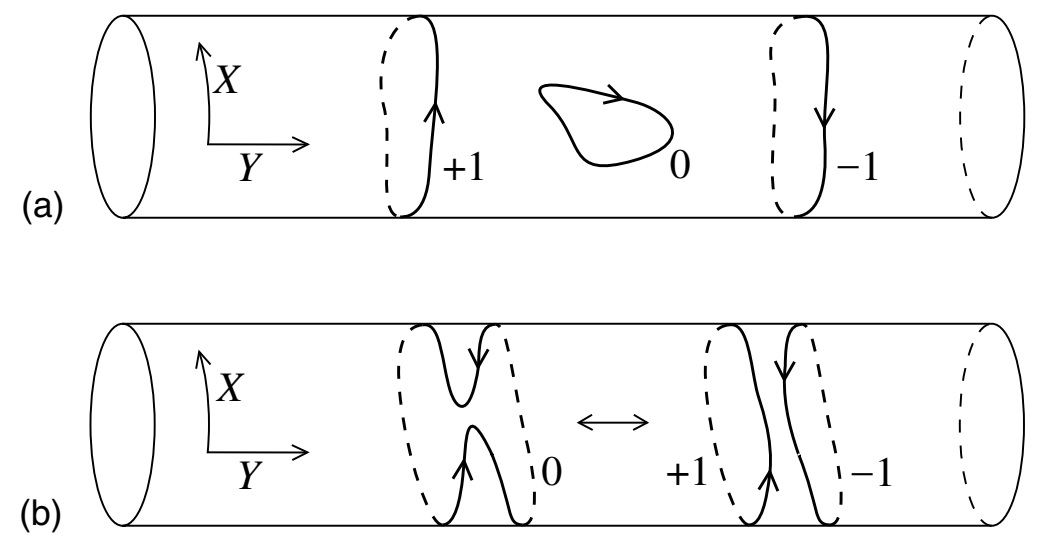
\includegraphics[width=0.8\textwidth,natwidth=789,natheight=408.75]{Fig8.1.jpg}\\
		\caption{(a) 缠绕数为$w=+1,0,-1$的定向闭弦. (b) $w=0$的弦跃迁至 $w=+1$ 和 $w=-1$ 的弦.}\label{Fig8.1}
	\end{center}
\end{figure}


其二为弦论特有. 闭弦现在必须缠绕紧致维,
\begin{equation}
	X(\sigma+2 \pi)=X(\sigma)+2 \pi R w, \quad w \in \mathds{Z} \:. \label{8.2.3}
\end{equation}
整数 $w$ 是缠绕数. 缠绕数为 $+1, 0 ,-1$的态如图\ref{Fig8.1}(a)所示.
从世界面场论的观点来看, 缠绕数非零的弦是拓扑孤子, 即场构型拓扑非平庸的态. 相容的弦理论必须纳入缠绕数态: 通过分裂-合并过程, 
$w=0$ 的弦可以变成 $w=+1$, $w=-1$ 的弦, 如图\ref{Fig8.1}(b)所示. 很容易看到这个例子中缠绕数总是守恒的. 

为了确定闭弦 CFT 的态, 考察洛朗展开
\begin{equation}
	\partial X(z)=-\mi\left(\frac{\alpha^{\prime}}{2}\right)^{1 / 2} \sum_{m=-\infty}^{\infty} \frac{\alpha_{m}}{z^{m+1}}\:, \qquad 
	\bar{\partial} X(\bar{z})=-\mi\left(\frac{\alpha^{\prime}}{2}\right)^{1 / 2} \sum_{m=-\infty}^{\infty} \frac{\tilde{\alpha}_{m}}{\bar{z}^{m+1}} \:. \label{8.2.4}
\end{equation}
缠绕一周后, $X$的改变为
\begin{equation}
	2 \pi R w=\oint(\dif z\: \partial X + \dif \bar{z}\: \bar{\partial} X)= 2 \pi(\alpha^{\prime}/2)^{1/2}(\alpha_{0}-\tilde{\alpha}_{0}) \:. \label{8.2.5}
\end{equation}
总的诺特动量是
\begin{equation}
	p=\frac{1}{2 \pi \alpha^{\prime}} \oint(\dif z\: \partial X- \dif \bar{z}\: \bar{\partial} X)
	=(2 \alpha^{\prime})^{-1 / 2}(\alpha_{0}+\tilde{\alpha}_{0}) \:. \label{8.2.6}
\end{equation}
对于非紧致维度, 这像往常一样给出 $\alpha_{0}=\tilde{\alpha}_{0}=p(\alpha^{\prime} / 2)^{1 / 2}$, 但对于周期维度则有
\begin{subequations} \label{8.2.7}
\begin{align}
p_{L} \equiv\left(2 / \alpha^{\prime}\right)^{1 / 2} \alpha_{0}=\frac{n}{R}+\frac{w R}{\alpha^{\prime}} \:, \label{8.2.7a} \\
p_{R} \equiv\left(2 / \alpha^{\prime}\right)^{1 / 2} \tilde{\alpha}_{0}=\frac{n}{R}-\frac{w R}{\alpha^{\prime}} \:. \label{8.2.7b}
\end{align}		
\end{subequations}
Virasoro生成元是
\begin{subequations} \label{8.2.8}
\begin{align}
L_{0}&=\frac{\alpha^{\prime} p_{L}^{2}}{4}+\sum_{n=1}^{\infty} \alpha_{-n} \alpha_{n} \:, \label{8.2.8a} \\
\tilde{L}_{0}&=\frac{\alpha^{\prime} p_{R}^{2}}{4}+\sum_{n=1}^{\infty} \tilde{\alpha}_{-n} \tilde{\alpha}_{n} \:. \label{8.2.8b}
\end{align}		 				
\end{subequations}


\subsection*{配分函数}
 $X$ 的配分函数
	\begin{align}
		&(q \bar{q})^{-1 / 24} \operatorname{Tr}\Bigl(q^{L_{0}} \bar{q}^{\tilde{L}_{0}}\Bigr) \nonumber \\
		&\quad =|\eta(\tau)|^{-2} \sum_{n, w=-\infty}^{\infty} q^{\alpha^{\prime} p_{L}^{2} / 4} \bar{q}^{\alpha^{\prime} p_{R}^{2} / 4} \nonumber \\
		&\quad =|\eta(\tau)|^{-2} \sum_{n, w=-\infty}^{\infty} \exp \left[-\pi \tau_{2}\left(\frac{\alpha^{\prime} n^{2}}{R^{2}}+\frac{w^{2} R^{2}}{\alpha^{\prime}}\right)+2 \pi \mi \tau_{1} n w\right] \:. \label{8.2.9}
	\end{align}
振子与非紧致情况相同, 而动量积分被换成了对$n$ 和 $w$的求和. 模不变性不显然, 但利用Poisson重求和公式,
\begin{equation}
	\sum_{n=-\infty}^{\infty} \exp (-\pi a n^{2}+2 \pi \mi b n)=a^{-1 / 2} 
	\sum_{m=-\infty}^{\infty} \exp \biggl[-\frac{\pi(m-b)^{2}}{a}\biggr] \:. \label{8.2.10}
\end{equation}
配分函数变成
\begin{equation}
	2 \pi R Z_{X}(\tau) \sum_{m, w=-\infty}^{\infty} \exp \biggl(-\frac{\pi R^{2}|m-w \tau|^{2}}{\alpha^{\prime} \tau_{2}}\biggr) \:. \label{8.2.11}
\end{equation}
% \fbox{\noindent\centering\parbox{0.9\textwidth}{Note:
% $$
% \begin{aligned}
% &\sum_{n=-\infty}^{+\infty} \exp \left[-\pi \tau_{2} \frac{\alpha^{\prime} n^{2}}{R^{2}}+2 \pi i \tau_{1} n w-\pi \tau_{2}  \frac{w^{2} R^{2}}{\alpha^{\prime}}\right] \\
% &=\frac{R}{\left(\alpha^{\prime} \tau_{2}\right)^{1 / 2}} \sum_{m=-\infty}^{+\infty} \exp \left[-\frac{\pi R^{2}}{\alpha^{\prime} \tau_{2}}\left(\left(m-w \tau_{1}\right)^{2}+w^{2} \tau_{2}^{2}\right)\right]
% \end{aligned}
% $$
% $$
% Z_{x}(\tau)=\frac{|\eta(\tau)|^{-2}}{\left(4 \pi^{2} \alpha^{\prime} \tau_{2}\right)^{1 / 2}}
% $$}}\\
$Z_{X}(\tau)$是非紧致理论中的模不变表达式\eqref{7.2.9}, 这个和在 $\tau \rightarrow \tau+1$下显然是不变的. 而当$\tau \rightarrow-1 / \tau$ 时, 它在$m\to-w$和$w\to m$下不变.

\begin{tcolorbox}
	\begin{remark}
		在$\tau \to -1/\tau$下, 
		\[
			\frac{|m-w \tau|^{2}}{\tau_{2}} \rightarrow \frac{| m+w / \tau|^{2}}{\tau_{2} /|\tau|^{2}}=\frac{|m \tau+w|^{2}}{\tau_{2}}	
		\]
	\end{remark}
\end{tcolorbox}


\eqref{8.2.11} 有一个简单的路径积分解释. 在周期时空中对所有亏格为1的世界面求和, 世界面上每个不平庸的闭曲线会缠绕紧致方向
\begin{subequations} \label{8.2.12}
\begin{align}
X(\sigma^{1}+2 \pi, \sigma^{2}) &= X(\sigma^{1}, \sigma^{2})+2 \pi w R \:, \label{8.2.12a} \\
X(\sigma^{1}+2 \pi \tau_{1}, \sigma^{2}+2 \pi \tau_{2}) &= X(\sigma^{1}, \sigma^{2})+2 \pi m R \:. \label{8.2.12b} 
\end{align}
\end{subequations}
即, 路径积分分裂成由$w$ 和 $m $标记的拓扑不等价截面. 通过将$X$写成满足周期性的经典解                                                                                                              
\begin{equation}
	X_{\mathrm{cl}}=\sigma^{1} w R+\sigma^{2}(m-w \tau_{1}) R / \tau_{2} \:, \label{8.2.13}
\end{equation}
加上满足周期性边界条件的量子部分. 这个高斯型路径积分可以积掉. 对量子部分的路径积分与非紧致情况相同, 而经典部分作为\eqref{8.2.11}中的指数出现. 
模变换在周期性上的效应就简化为交换求和变量 $m$ 和 $w$.

\subsection*{顶点算符}
为了构造 $\alpha_{0} \neq \tilde{\alpha}_{0}$的缠绕态, 我们需要独立的变量 $x_{L}$和 $x_{R}$, 满足
\begin{equation}
	[x_{L}, p_{L}]=[x_{R}, p_{R}]=\mi \:. \label{8.2.14}
\end{equation}
场 $X$ 分裂成称全纯部分和反全纯部分
\begin{equation}
	X(z, \bar{z})=X_{L}(z)+X_{R}(\bar{z}) \:, \label{8.2.15}
\end{equation}
其中
\begin{subequations} \label{8.2.16}
\begin{align}
X_{L}(z) &= x_{L}- \mi \frac{\alpha^{\prime}}{2} p_{L} \ln z+\mi\left(\frac{\alpha^{\prime}}{2}\right)^{1 / 2} 
			\sum_{\substack{m=-\infty  \\  m \neq 0}}^{\infty} \frac{\alpha_{m}}{m z^{m}} \:, \label{8.2.16a} \\
X_{R}(\bar{z})&= x_{R}-\mi \frac{\alpha^{\prime}}{2} p_{R} \ln \bar{z}+\mi\left(\frac{\alpha^{\prime}}{2}\right)^{1 / 2} 
\sum_{\substack{m=-\infty  \\  m \neq 0}}^{\infty} \frac{\tilde{\alpha}_{m}}{m \bar{z}^{m}} \:. \label{8.2.16b}
\end{align}
\end{subequations}
如果我们限制在 $k_{L}=k_{R}$的态上且只用 $X_{L}(z)+X_{R}(\bar{z})$构建的算符, 这就退化至非紧致维度的CFT.

我们现在讨论OPE与顶点算符. 很容易猜出顶点算符的形式, 既然通常的$XX$算符乘积 $-(\alpha^{\prime} / 2) \ln (z_{12} \bar{z}_{12})$可以拆成全纯函数和反全纯函数, 因此
\begin{subequations} \label{8.2.17}
\begin{align}
X_{L}(z_{1}) X_{L}(z_{2}) &\sim-\frac{\alpha^{\prime}}{2} \ln z_{12}, \quad 
X_{R}(\bar{z}_{1}) X_{R}(\bar{z}_{2}) \sim-\frac{\alpha^{\prime}}{2} \ln \bar{z}_{12}  \:,  \label{8.2.17a} \\
X_{L}(z_{1}) X_{R}(\bar{z}_{2}) &\sim 0 \:. \label{8.2.17b}
\end{align}		
\end{subequations}
对应于态 $|0 ; k_{L}, k_{R}\rangle$的算符是
\begin{equation}
	\mathscr{V}_{k_{L} k_{R}}(z, \bar{z}) = : \mathrel{e^{\mi k_{L} X_{L}(z)+ \mi k_{R} X_{R}(\bar{z})}}: \label{8.2.18}
\end{equation}
OPE为
\begin{equation}
	\mathscr{V}_{k_{L} k_{R}}(z_{1}, \bar{z}_{1}) \mathscr{V}_{k_{L}^{\prime} k_{R}^{\prime}}(z_{2}, \bar{z}_{2}) \sim 
	z_{12}^{\alpha^{\prime} k_{L} k_{L}^{\prime} / 2} \bar{z}_{12}^{\alpha^{\prime} k_{R} k_{R}^{\prime} / 2} 
	\mathscr{V}_{(k+k^{\prime})_{L}(k+k^{\prime})_{R}}(z_{2}, \bar{z}_{2}) \:. \label{8.2.19}
\end{equation}
我们会在各种表达式中遇到支点、割线, 这不奇怪, 因为场$X$不再是单值的. 然而重要的是, 整个顶点算符的OPE必须是单值的: 当 $z_{1}$ 环绕 $z_{2}$一周, 净相位为1.
\begin{equation}
	\exp [\pi \mi \alpha^{\prime}(k_{L} k_{L}^{\prime}-k_{R} k_{R}^{\prime})]
	=\exp [2 \pi \mi(n w^{\prime}+w n^{\prime})]=1 \:. \label{8.2.20}
\end{equation}
为了使弦振幅合理定义, 这正是所必须的.

% \fbox{\noindent\centering\parbox{0.9\textwidth}{Note:
% 		$$
% 		k_{L} \cdot k_{L}^{\prime}=\left(\frac{n}{R}+\frac{w R}{\alpha^{\prime}}\right)\left(\frac{n^{\prime}}{R}+\frac{w^{\prime} R}{\alpha^{\prime}}\right)=\frac{n n^{\prime}}{R^{2}}+\frac{w^{\prime} n}{\alpha^{\prime}}+\frac{n w^{\prime} }{\alpha^{\prime}}+\frac{w w^{\prime} R^2}{(\alpha^\prime)^2}
% 		$$
% 	$$
% 	k_{R} \cdot k_{R}^{\prime}=\left(\frac{n}{R}-\frac{w R}{\alpha^{\prime}}\right)\left(\frac{n^{\prime}}{R}-\frac{w^{\prime} R}{\alpha^{\prime}}\right)=\frac{n n^{\prime}}{R^{2}}-\frac{w^{\prime} n}{\alpha^{\prime}}-\frac{n w^{\prime} }{\alpha^{\prime}}+\frac{w w^{\prime} R^2}{(\alpha^\prime)^2}
% 	$$
% $$
% \alpha^{\prime}\left(k_{L} \cdot k_{L}^{\prime}-k_{R} k_{R}^{\prime}\right)=2 w^{\prime} n+2 n w^{\prime}
% $$}}\\


\subsection*{一个技巧}

前面的讨论显然是正确的, 但我们对于对数中支点、割线位置的处理太过随便. 如果我们交换$z_{1}$ 和 $z_{2}$, 以及动量 $k$ 和 $k^{\prime} $, 
OPE\eqref{8.2.19}就会出现问题. 左边是对称的, 但右边会差 $\exp[\pi \mi(n w^{\prime}+w n^{\prime})]$. 因此, 
如果 $n w^{\prime}+w n^{\prime}$为奇, 会差一个负号. 我们也可以以如下方式看到这个问题. 从模展开可导出等时 $(|z_{1}|=|z_{2}|)$ 对易子
\begin{equation}
	[X_{L}(z_{1}), X_{L}(z_{2})]=\frac{\pi \mi \alpha^{\prime}}{2} \operatorname{sign}(\sigma_{1}^{1}-\sigma_{2}^{1}) \:. \label{8.2.21}
\end{equation}
那么CBH公式告诉我们, 如果我们通过产生-湮灭次序定义算符, 那么$n w^{\prime}+w n^{\prime}$ 为奇时, 算符 $\mathscr{V}_{k_{L} k_{R}}$ 与 $\mathscr{V}_{k_{k}^{\prime} k_{R}^{\prime}}$反对易; 不可见的支点、割线\eqref{8.2.20}会变成两个可视的. 顶点算符正确的振子表达式是(相位中有任意性) 
\begin{equation}
	\mathscr{V}_{k_{L} k_{R}}(z, \bar{z})=\exp [\pi \mi(k_{L}-k_{R})(p_{L}+p_{R}) \alpha^{\prime} / 4] 
	\mathrel{\typecolon \me^{\mi k_{L} X_{L}(z)+\mi k_{R} X_{R}(\bar{z})} \typecolon} \:, \label{8.2.22}
\end{equation}
其中像往常一样,  $p_L,p_R$ 是算符, $k$ 是数 (给定顶点算符携带的动量). 
当 $\mathscr{V}_{k_{L} k_{R}}$和 $\mathscr{V}_{k_{L}^{\prime} k_{R}^{\prime}}$彼此对易时, 额外的因子称为闭上链(cocycles), 这给出额外相位
\begin{align}
	\exp \Bigl\{\pi \mi\Bigl[(k_{L}-k_{R})(k_{L}^{\prime}+k_{R}^{\prime})-(k_{L}^{\prime}-k_{R}^{\prime})(k_{L}+k_{R})\Bigr] 
	\alpha^{\prime} / 4\Bigr\}\quad &  \nonumber \\
	=\exp [\pi \mi(n w^{\prime}-w n^{\prime})] &\:, \label{8.2.23}
\end{align}
这移除了支点、割线. 对于大多数情况, 可以忽视这一复杂性, 并用上一段那个更简单的表达式进行处理; 闭上链只影响特定振幅的相对符号.

一般的 $X^{\mu}$ 路径积分 \eqref{6.2.18} 以一种显然的方式因式分解成全纯和反全纯的, 这使得我们可以做替换
\begin{equation}
	\prod_{i<j}^{n}|z_{i j}|^{\alpha^{\prime} k_{i} k_{j}} \to \prod_{i<j}^{n} z_{i j}^{\alpha^{\prime} k_{L i} k_{L j} / 2} 
	\bar{z}_{i j}^{\alpha^{\prime} k_{R i} k_{R j} / 2} \:, \label{8.2.24}
\end{equation}
也可将来自 $x_{0}$的非紧致积分的 $2 \pi \delta(\sum k)$ 换成
\begin{equation}
	2 \pi R \delta_{\Sigma_{i} n_{i}, 0} \delta_{\Sigma_{i} w_{i}, 0} \:. \label{8.2.25}
\end{equation}
精确表达式 \eqref{8.2.22} 会给出一些额外的符号.

\subsection*{DDF算符}

我们已经看到指数算符可以分成全纯和反全纯部分, 这有很多应用, 我们现在用它来讨论第4章末尾的DDF算符.

我们将用光锥坐标 $X^{\pm}=2^{-1 / 2}(X^{0} \pm X^{1})$处理, 它的全纯部分有 OPE(扔掉下标 $L$)
\begin{equation}
	X^{+}(z) X^{-}(0) \sim \frac{\alpha^{\prime}}{2} \ln z, \qquad X^{+}(z) X^{+}(0) \sim X^{-}(z) X^{-}(0) \sim 0 \:. \label{8.2.26}
\end{equation}
\begin{tcolorbox}
	\begin{remark}
		\begin{align*}
X^{+}(z) X^{-}(0) &=2^{-1}\left(X^{0}(z)+X^{\prime}(z)\right)\left(X^{0}(0)-X^{\prime}(0)\right) \\
&=2^{-1}\left(\frac{\alpha^{\prime}}{2} \ln z_{12}+\frac{\alpha^{\prime}}{2}\ln z_{12}\right)=\frac{\alpha^{\prime}}{2} \ln z_{12} \:.
		\end{align*}
	\end{remark}
\end{tcolorbox}
\noindent 由此得出算符
\begin{equation}
	V^{i}(n k_{0}, z)=\partial X^{i}(z) \me^{\mi n k_{0} X^{+}(z)}(2 / \alpha^{\prime})^{1 / 2} \label{8.2.27}
\end{equation}
是$(1,0)$本原场, 其中$i$是横向指标. OPE 为
\begin{align}
	V^{i}(n k_{0}, z) V^{j}(m k_{0}, 0) &\sim-\frac{\delta^{i j}}{z^{2}} \me^{\mi(n+m) k_{0} X^{+}(0)}  \nonumber \\
	&\quad -\frac{\mi n k_{0} \delta^{i j}}{z} \partial X^{+}(0) \me^{\mi(n+m) k_{0} X^{+}(0)} \:. \label{8.2.28}
\end{align}
定义DDF算符为
\begin{equation}
	A_{n}^{i}=\oint \frac{\dif z}{2 \pi} \, V^{i}(n k_{0}, z) \:. \label{8.2.29}
\end{equation}
除非$n+m=0$, 否则OPE\eqref{8.2.28}中的 $z^{-1}$ 项就是全导数, 因而 DDF 算符满足振子代数
\begin{equation}
	[A_{m}^{i}, A_{n}^{j}]=m \delta^{i j} \delta_{m,-n} \frac{\alpha^{\prime} k_{0} p^{+}}{2} \:. \label{8.2.30}
\end{equation}

考察这个算符在动量给定为 $q$的态上的作用.  $V^{i}(n k_{0}, z)$ 与这个态的顶点算符将会包含 $z^{-\alpha^{\prime} n k_{0} q^{-} / 2}$. 
因而如果我们固定$k_{0}=2 / \alpha^{\prime} q^{-}$, 它将是单值的. 那么围道积分\eqref{8.2.29}就在这个截面上定义了合理的算符. 
DDF 算符是 $(1,0)$张量的积分, 因而与Virasoro生成元对易, 它将物理态变到物理态. 由此, 我们可以通过用 DDF 算符作用振子基态建立物理态. 
以这种方法得到的态与光锥态一一对应. DDF算符不包含$X^{-}$, 因而这些态没有 $\alpha_{-m}^{-}$激发. 
因此, 与更加一般但不太显然的构造\eqref{4.4.19}相比, 它们实际上给出相同的态.


\section{闭弦和T对偶} \label{sec:8.3}%{8.3 Closed strings and T -duality}

既然我们在研究弦理论, 我们取 $D=26$, 并且只取 $X^{25}$ 是周期的. 质壳 ($L_{0}$与$\tilde{L}_{0}$) 是
	\begin{align}
		m^{2}=-k^{\mu} k_{\mu} &= (k_{L}^{25})^{2}+\frac{4}{\alpha^{\prime}}(N-1) \nonumber \\
		&=(k_{R}^{25})^{2}+\frac{4}{\alpha^{\prime}}(\tilde{N}-1) \:, \label{8.3.1}
	\end{align}
或
\begin{subequations} \label{8.3.2}
\begin{align}
m^{2} &= \frac{n^{2}}{R^{2}}+\frac{w^{2} R^{2}}{\alpha^{\prime 2}}+\frac{2}{\alpha^{\prime}}(N+\tilde{N}-2) \:, \label{8.3.2a} \\
0 &= n w+N-\tilde{N} \:. \label{8.3.2b} 
\end{align}
\end{subequations}
对质量平方有四个贡献: 紧致动量, 缠绕弦的势能, 振子以及零点能. 第\ref{cha:4}章对物理频谱的讨论适用于任何紧致化, 
所以我们仅通过考察横向振子 $M=2, \ldots, 25$, 就得到了态的正确计数.

首先, 我们复现出无质量频谱的场论结果. 在$R$的一般值处, 仅当$n=w=0$, $N=\tilde{N}=1$时, 态才可能是无质量的. 这里有 $24^{2}$个相同的态, 但是根据振子是处在时空方向 $\mu$还是内部方向25, 对其分类将是有用的:
\begin{align}
	&\alpha_{-1}^{\mu} \tilde{\alpha}_{-1}^{\nu}|0 ; k\rangle\:, \qquad 
	(\alpha_{-1}^{\mu} \tilde{\alpha}_{-1}^{25}+\alpha_{-1}^{25} \tilde{\alpha}_{-1}^{\mu})|0 ; k\rangle \:, \nonumber \\
	&(\alpha_{-1}^{\mu} \tilde{\alpha}_{-1}^{25}-\alpha_{-1}^{25} \tilde{\alpha}_{-1}^{\mu})|0 ; k\rangle\:, \qquad 
	\alpha_{-1}^{25} \tilde{\alpha}_{-1}^{25}|0 ; k\rangle \:. \label{8.3.3}
\end{align}
其中第一个进一步分裂成25维引力子加伸缩子加反对称张量. 第二个, 时空维度与内部指标上的引力子, 它是Kaluza-Klein矢量. 第三个是来自反对称张量的矢量. 
最后一个态是标量, 它是紧致方向上半径的模, 它的顶点算符 $:\mathrel{\partial X^{25} \bar{\partial} X^{25} \me^{\mi k \cdot X}}:$ 是度规 $G_{25,25}$的微扰. 这与考察低能场论时发现的频谱相同.

考察有质量的态在 $U(1) \times U(1)$ 对称性下的变换是十分有益的. 再一次, Kaluza-Klein 规范对称性来自 $X^{25}$ 方向上的平移, 
所以相应的荷是紧致动量 $p_{25} $. 对于反对称张量规范对称性, 考察零动量顶点算符, 它测出了任何与其耦合的态的变换. 它正比于
\begin{equation}
	\partial X^{\mu} \bar{\partial} X^{25}-\partial X^{25} \bar{\partial} X^{\mu}= 
	\bar{\partial}(X^{25} \partial X^{\mu})-\partial(X^{25} \bar{\partial} X^{\mu}) \:. \label{8.3.4}
\end{equation}
这是全导数, 但是在缠绕态上, 由于$X^{25}$不是单值的, 所以它的积分不为零. 所以 $B_{\mu, 25}$荷是缠绕数. 
这是这一紧致化中我们首个遇到的``弦''物理: 在场论中没有携带这一荷的态.

我们从弦三点耦合来验证规范耦合. 规范玻色子顶点算符是
\begin{equation}
	\frac{2^{1 / 2} g_{\mathrm{c}, 25}}{\alpha^{\prime}}:\mathrel{(\partial X^{\mu} \bar{\partial} X^{25} \pm 
	\partial X^{25} \bar{\partial} X^{\mu}) \me^{\mi k \cdot X}}: \:. \label{8.3.5}
\end{equation}
我们将25维弦耦合 $g_{\mathrm{c}, 25}=g_{\mathrm{c}}(2 \pi R)^{-1 / 2}$. 因子 $(2 \pi R)^{-1 / 2}$ 来自于零模波函数的归一化, 
对于一般的紧致动量和缠绕数, 快子的顶点算符是
\begin{equation}
	g_{\mathrm{c}, 25}:\mathrel{ \me^{\mi k_{L} \cdot X_{L}(z)+\mi k_{R} \cdot X_{R}(\bar{z})}}: \:.
\end{equation}
一个规范玻色子与两个快子的三点振幅, 若快子的紧致动量以及缠绕数不为零, 那么类似于\eqref{6.6.14},
\begin{align}
	& {-}2^{-1 / 2} \pi \mi g_{\mathrm{c}, 25}(2 \pi)^{25} \delta^{25}({\textstyle\sum_{i} k_{i}}) k_{23}^{\mu}
	(k_{L 23}^{25} \pm k_{R 23}^{25}) \nonumber \\
	\to & {-}2^{3 / 2} \pi \mi g_{\mathrm{c}, 25}(2 \pi)^{25} \delta^{25}({\textstyle \sum_{i} k_{i}}) k_{2}^{\mu}
	(k_{L 2}^{25} \pm k_{R 2}^{25}) \:. \label{8.3.7}
\end{align}
在第二行, 我们取规范玻色子动量 $k_{1} \rightarrow 0$, 这定义了规范耦合. 两个规范玻色子分别与 $k_{L 2}^{25} \pm k_{R 2}^{25}$耦合, 即紧致动量与缠绕数. 
这正是我们期待的. 将规范玻色子换成引力子, 继续考察这个振幅, 我们将复现出各个耦合间的关系\eqref{8.1.11}, \eqref{8.1.12}, 这与有效作用量中发现的是相同的.

\subsection*{增强的规范对称性}

迄今为止, 所有事情都与一个维度紧致化的场论完全相同. 26维引力子产生了25维引力子加矢量加模. 唯一的弦效应是携带 $B_{\mu, 25}$荷的缠绕态.

进一步且更神奇的效应来自于特殊的紧致半径. 我们对无质量频谱的讨论省略了, 仅对半径$R $的特殊值, 态才是无质量的. 最丰富的情况是$R=\alpha^{1 / 2}$, 
这样 $k_{L, R}^{25}=(n \pm w) \alpha^{\prime-1 / 2}$, 而无质量态的条件是
\begin{equation}
	(n+w)^{2}+4 N=(n-w)^{2}+4 \tilde{N}=4 \:. \label{8.3.8}
\end{equation}
除了一般解$n=w=0, N=\tilde{N}=1$, 现在还有
\begin{equation}
	n=w=\pm 1,\: N=0,\: \tilde{N}=1\:, \quad n=-w=\pm 1, \: N=1, \:\tilde{N}=0 \:, \label{8.3.9}
\end{equation}
以及
\begin{equation}
	n=\pm 2,\: w=N=\tilde{N}=0\:, \quad w=\pm 2, \: n=N=\tilde{N}=0 \:. \label{8.3.10}
\end{equation}

态 \eqref{8.3.9} 引入了4个规范玻色子, 其顶点算符
\begin{equation}
	: \mathrel{\bar{\partial} X^{\mu} \me^{\mi k \cdot X} \exp [\pm 2 \mi \alpha^{\prime-1 / 2} X_{L}^{25}]}: \:, \quad 
	: \mathrel{ \partial X^{\mu} \me^{\mi k \cdot X} \exp [\pm 2 \mi \alpha^{\prime-1 / 2} X_{R}^{25}]}: \:. \label{8.3.11}
\end{equation}
指数算符精确定义与上节相同. 这些态拥有内部动量与缠绕数, 所以它们携带 Kaluza-Klein 荷以及反对称张量规范荷. 带荷的无质量矢量的唯一相容理论是非阿贝尔规范理论, 
所以新的规范玻色子必须与旧有规范玻色子结合形成非阿贝尔理论. 现在用 $\partial X^{25} \bar{\partial} X^{\mu}$ 和 $\partial X^{\mu} \bar{\partial} X^{25}$ 处理之前的矢量将是方便的. 其中第一个与$k_{L}^{25}$耦合, 在这个耦合下, \eqref{8.3.11}中的第一对态携带荷 $\pm 1$, 而第二对是中性的. 
第二个与 $k_{R}^{25}$ 耦合, 其它类似. 这表明规范群是 $S U(2) \times S U(2)$, 那三个包含 $\bar{\partial} X^{\mu}$ 的矢量构成 $S U(2)$. 
而另三个则构成另一个 $S U(2)$. 

为了呈现这个$S U(2) \times S U(2)$, 定义3个$(1,0)$流
\begin{subequations} \label{8.3.12}
\begin{align}
j^{1}(z)&=: \mathrel{\cos [2 \alpha^{-1 / 2} X_{L}^{25}(z)]}: \:, \label{8.3.12a}  \\
j^{2}(z)&=:\mathrel{ \sin [2 \alpha^{\prime-1 / 2} X_{L}^{25}(z)]}: \:, \label{8.3.12b} \\
j^{3}(z)&=\mi \partial X_{L}^{25}(z) / \alpha^{\prime 1 / 2} \:. \label{8.3.12c}
\end{align}
\end{subequations}
它们可以被归一化, 使得 OPE
\begin{equation}
	j^{i}(z) j^{j}(0) \sim \frac{\delta^{i j}}{2 z^{2}}+ \mi \frac{\epsilon^{i j k}}{z} j^{k}(0) \:. \label{8.3.13}
\end{equation}
对于 $(0,1)$ 流 $\tilde{\jmath}^{i} $, 有类似的OPE. 单极点项暗示了相应的荷构成 $SU(2)$ 代数. 实际上, 既然这些流是全纯的, 存在由洛朗系数构成的无限维代数
\begin{subequations} \label{8.3.14}
\begin{align}
		j^{i}(z) &= \sum_{m=-\infty}^{\infty} \frac{j_{m}^{i}}{z^{m+1}}  \:, \label{8.3.14a} \\
		[j_{m}^{i}, j_{n}^{j}] &= \frac{m}{2} \delta_{m,-n} \delta^{i j}+ \mi \epsilon^{i j k} j_{m+n}^{k} \:, \label{8.3.14b} 
\end{align}
\end{subequations}
这被称为流代数, 仿射李代数, 或 Kac-Moody 代数. 我们会在第\ref{cha:11}章开头频繁地遇到这样的代数. 将会证明 $z^{-2}$ 的系数是量子化的, 
而\eqref{8.3.13}中的值是最小值. 所以这被称为一阶 $SU(2)$ 流代数.

这一 $S U(2) \times S U(2)$ 对称性首次表明了弦论看到时空几何方式与我们在场论中所用的完全不同, 
在场论中只有 $U(1) \times U(1)$ 对称性在任意半径下都是显然的.  $j^{3}$ 与 $j^{1,2}$ 的起源完全不同, 它们分别是振子激发和缠绕数-动量激发, 
它们表示成 $X^{25}$ 的形式也完全不同, 但是在它们对弦频谱的作用中, 它们通过对称性彼此相关. 由于内动量和缠绕数的能量被负的零点能抵消了, 额外的矢量是无质量的. 
这种情况不仅发生在快子理论中, 在卷II还会有其他情况.

\subsection*{标度与耦合}

在 $S U(2) \times S U(2)$ 半径, 关系\eqref{8.1.11}变成
\footnote{精确些, 这是一个 $(n, w)=(1,0)$ 态的耦合. 非阿贝尔规范子有$(|n|,|w|)=(1,1)$, 
所以它们的耦合是$g_{S U(2), 25}^{2}=4 \kappa_{25}^{2} / \alpha^{\prime}$, 这是传统量子物理对$SU(2)$耦合的定义. 
我们会在第18章看到这对所有一阶流代数都成立.}
\begin{equation}
	g_{25}^{2}=2 \kappa_{25}^{2} / \alpha^{\prime} \:. \label{8.3.15}
\end{equation}
如果我们对多个维度做紧致化, 每个维度以相同方式重新标度. 所以, 特别地, 在4维中
\begin{equation}
	g_{4}^{2}=2 \kappa_{4}^{2} / \alpha^{\prime} \:. \label{8.3.16}
\end{equation}
在自然界中, 非阿贝尔规范耦合的量级在1左右, 这暗示了弦长 $\alpha^{1 / 2}$与引力长度 $\kappa_{4}$相差不远.

我们也可以如下方式思考此事. 4维规范耦合无量纲, 但4维引力耦合有量纲. 定义有效无量纲引力耦合, 它依赖于能量标度 $E$,
\begin{equation}
	g_{\mathrm{G}, 4}^{2}(E)=\kappa_{4}^{2} E^{2} \:, \label{8.3.17}
\end{equation}
它随着能量平方增长. 显然, 无量纲规范耦合随着能量跑动, 但这又慢于引力耦合的量纲标度. 那么通过\eqref{8.3.16}, 弦的质量标度是规范与引力耦合粗略相等的地方, 
$g_{\mathrm{G}, 4}^{2}(E) \approx g_{4}^{2}$.

同样有益的是考察紧致化到4维的可能性, 其中的一些紧致化维度可能远大于另一些. 这最好通过从低能开始然后向上进发进行分析, 在低能存在无量纲规范耦合 $g_{4}^{2}$. 
在能量 $\rho_{5}^{-1}$, 一个紧致维度变成可见维度, 而物理变成5维(简单起见, 我们在这一标度下只考察这一个维度). 有效5维耦合是
\begin{equation}
	g_{5}^{2}=2 \pi \rho_{5} g_{4}^{2} \:. \label{8.3.18}
\end{equation}
和\eqref{8.1.12}一样, 这源于有效作用量. 耦合 $g_{5}^{2}$ 有长度量纲. 即, 5维杨-米尔斯理论, 同4维引力一样, 不可重整. 相应的, 有效无量纲耦合是
\begin{equation}
	\hat{g}_{5}^{2}=g_{5}^{2} E=2 \pi \rho_{5} E g_{4}^{2} \:, \label{8.3.19}
\end{equation}
它随能量线性增长. 然而 $g_{4}^{2}$在自然界并非远小于1, 所以耦合在高能处很快变强; 据推测, 这时就需弦论使得短距行为变得合理. 
所以这一紧致化标度必须接近于引力标度. 这种分析在开弦理论中被修正了, 而在那时, 在强耦合弦理论的现代理解被考虑在内. 
有非常低的可能性, 弦或 Kaluza-Klein 激发远低于普朗克标度.

\subsection*{Higgs机制}
令$R$远离 $S U(2) \times S U(2)$ 半径. 考察会发生什么是最有启发性的. 额外的规范玻色子现在获得质量
\begin{equation}
	m=\frac{|R^{2}-\alpha^{\prime}|}{R \alpha^{\prime}} \approx \frac{2}{\alpha^{\prime}}\Bigl|R-\alpha^{\prime 1 / 2}\Bigr| \:, 
	\label{8.3.20}
\end{equation}
这一近似是半径$R$很接近于 $S U(2) \times S U(2)$半径 $\alpha^{\prime 1 / 2}$ . 在这一半径附近, 质量远小于弦标度, 我们应该用低能场论来理解物理.

只有一种方式能赋予规范玻色子这样的质量, 自发对称性破缺, 这正是所发生的. 当 $R=\alpha^{1 / 2}$, 存在10个无质量标量, 伸缩子, 模 $G_{25,25}$, 
\eqref{8.3.9}中的4个态, 以及 \eqref{8.3.10}中的4个态, 后9个由如下的顶点算符产生
\begin{equation}
	: \mathrel{j^{i}(z) \tilde{\jmath}^{j}(\bar{z}) \me^{\mi k \cdot X(z, \bar{z})}}: \:. \label{8.3.21}
\end{equation}
指标$i$ 是左移 $SU(2)$ 下的矢量, 指标 $j$ 是右移$SU(2)$下的矢量. 即, 它们在$S U(2) \times S U(2) $下按照 $(\bm{3},\bm{3})$表示变换. 
特别地, 半径的模是 $j^{3} \tilde{\jmath}^{3}$. 远离 $S U(2) \times S U(2)$半径会给予这个场期望值, 
所以将规范对称性破缺至保持$z$轴不变的$U(1) \times U(1)$对称性. 诚然, 这正是一般半径时的规范群. 在 $SU(2)$半径附近, 
质量 \eqref{8.3.20} 关于模的量纲 $|R-\alpha^{\prime 1 / 2}|$是是线性的, 这和通常的自发破缺一样. 

我们把与这9个标量场相对应的时空场记作$M_{i j} $. 模中的一变化是$M_{33} \neq 0$, 但是在 $S U(2) \times S U(2)$点附近, 对更一般的背景做些调查是很有启发性的. 这些无质量场的相互作用会由某个时空作用量进行描述, 而这个作用量会包含一个势$U(M)$. 这些场在对称点没有质量, 所以$U$中没有$M^{2}$项, 
但可能有 $(S U(2) \times S U(2))$不变的立方项
\begin{equation}
	U(M) \propto \epsilon^{i j k} \epsilon^{i^{i} j^{\prime} k^{\prime}} M_{i i^{\prime}} M_{j j^{\prime}} M_{k k^{\prime}}=\operatorname{det} M \:. \label{8.3.22}
\end{equation}
从弦的三点振幅不难证明这一项确实存在. 它是玻色子的三次项无下界, 但同快子一样, 这是玻色弦论的人工产物.

忽略这个势对小变分不稳定的事实, 寻找它的静态经典解是有意义的. 为了拥有静态背景解, 引力子与伸缩子的场方程要求势为零, 而$M_{i j}$ 的场方程要求势是稳定的
\begin{equation}
	U(M)=\frac{\partial U(M)}{\partial M_{i j}}=0 \:. \label{8.3.23}
\end{equation}
利用$S U(2) \times S U(2)$ 旋转对角化 $M$, 条件\eqref{8.3.23}变成
\begin{equation}
	M_{11} M_{22} M_{33}=M_{11} M_{22}=M_{11} M_{33}=M_{22} M_{33}=0 \:. \label{8.3.24}
\end{equation}
因此, 只能有一个对角分量可以不为零. 通过 $S U(2) \times S U(2)$转动, 我们可以取这个非零对角分量为$M_{33} $. 所以我们没构建任何物理的新的弦背景.

静态背景解的连续族称为平坦方向. 这里有9个无质量标量, 它们可以通过 $S U(2) \times S U(2)$ 旋转约化至3个对角场, 但是只有一个平坦方向 (规范等价的方向没有算进来). 当然, 我们只计算了场中的立方项, 但在一般情况下, 三次项可以为零. 而高次项依旧非零. 为了构建一个精确的平坦方向, 我们还需要更加专门的讨论. 
即, 对于任意的$R$值, 我们可以构建出自由 CFT. 注意到如果我们将 $j^{1} \tilde{\jmath}^{1}$或 $j^{2} \tilde{\jmath}^{2}$ 视为模, 
由于它们是$X^{25}$的正弦和余弦, 世界面作用量看起来会非常复杂, 但是由于它等价于变分$R$获得的自由理论, 所以世界面理论是可解的.

\subsection*{$T$对偶}
从质量公式
\begin{equation}
	m^{2}=\frac{n^{2}}{R^{2}}+\frac{w^{2} R^{2}}{\alpha^{\prime 2}}+\frac{2}{\alpha^{\prime}}(N+\tilde{N}-2) \:, \label{8.3.25}
\end{equation}
我们看到随着 $R \rightarrow \infty$, 缠绕态的质量变成无限大, 而紧致动量趋于连续谱, 这正是对于非紧致维度所预期的. 考察相反的极限 $R \rightarrow 0$. 
有紧致动量的态拥有了无穷大的质量, 但是缠绕态的频谱现在趋于连续——将弦缠绕在小圆上不会耗费太多的能量. 因此, 随着半径趋于零, 频谱同非紧致维度一样又一次趋于连续. 
这和场论行为完全不同, 在场论中只有紧致动量$n$ 没有缠绕数 $w$, 并且在$R \rightarrow 0$时, 没有态变轻.

事实上,  $R \rightarrow 0$和$R \rightarrow \infty$ 的极限在物理上是等价的. 频谱 \eqref{8.3.25} 在如下变换下不变
\begin{equation}
	R \rightarrow R^{\prime}=\frac{\alpha^{\prime}}{R}, \quad n \leftrightarrow w \:. \label{8.3.26}
\end{equation}
这一等价性同时扩展至相互作用. 注意调换 $n$和 $w$ 等价于
\begin{equation}
	p_{L}^{25} \rightarrow p_{L}^{25}\:, \quad p_{R}^{25} \rightarrow-p_{R}^{25} \:. \label{8.3.27}
\end{equation}
在半径 $R$处考察这个理论. 回忆分解$X^{25}(z, \bar{z})=X_{L}^{25}(z)+X_{R}^{25}(\bar{z})$, 定义
\begin{equation}
	X^{\prime 25}(z, \bar{z})=X_{L}^{25}(z)-X_{R}^{25}(\bar{z}) \:. \label{8.3.28}
\end{equation}
场$X^{\prime 25}$ 的OPE和能动张量与$X^{25}$的相同, 负号总会成对出现. 用 $X^{\prime 25}$替换 $X^{25}$ 对 CFT 造成的唯一改变是它引起了符号变化
\eqref{8.3.27}, 而这将为半径为 $R$的理论的频谱转化成半径为 $R^{\prime}$的理论的频谱. 即, 它们是相同的理论, 只不过一个写成$X^{25}$, 
另一个写成$X^{\prime 25} $.

这种等价性称为 $T$对偶. 即 $R \rightarrow 0$ 极限与 $R \rightarrow \infty$ 在物理上完全等价, 这与点粒子的行为完全不同, 
这也是在短程的弦的几何完全不同的又一佐证. 不等价理论的空间是射线$R \geq \alpha^{\prime 1 / 2} $. 
我们也可将范围取成$0 \leq R \leq \alpha^{1 / 2}$, 但是取较大的那个更自然些: 对我们而言, 动量连续区要比缠绕连续区更熟悉. 
并且在$R$较大的图景(picture)下, 定域性的问题会更加清楚. 因此, 最小的半径是自对偶半径
\begin{equation}
	R_{\text{自对偶}}=R_{SU(2) \times SU(2)}=\alpha^{\prime 1/2} \:. \label{8.3.29}
\end{equation}
最小距离尺度是弦长量级. 这一现象会在弦微扰论中反复出现, 但是非微扰地, 我们会看到尺度更小的结构. 

$T$ 对偶的很多应用体现在它对弦伸缩子$\Phi$的非平庸作用. 考察既无缠绕又无紧致动量的引力子的散射振幅. 这些态在$T$对偶下不变, 所以振幅也必须如此. 
后者可以从低能作用量\eqref{8.1.9}读出, 所以25维耦合 $\kappa_{25}$必须在对偶下不变. 而26维耦合 $\kappa=(2 \pi \rho)^{1 / 2} \kappa_{25}$, 
对偶的作用为
\begin{equation}
	\rho^{\prime}=\frac{\alpha^{\prime}}{\rho}\:, \qquad \kappa^{\prime}=\frac{\alpha^{\prime 1 / 2}}{\rho} \kappa \:. \label{8.3.30}
\end{equation}
既然 $\kappa \propto \me^{\Phi}$, 这暗示
\begin{equation}
	\me^{\Phi^{\prime}}=\frac{\alpha^{1 / 2}}{\rho} \me^{\Phi} \:. \label{8.3.31}
\end{equation}

$T$对偶是一种对称性, 它将单个理论中的不同态(背景)关联起来, 事实上, 它是规范对称性. 我们看到模 $\delta R$ 是 $(\bm{3},\bm{3})$场的33-分量. 
绕其中一个$S U(2)$ 的1-轴旋转 $\pi$角会反射模的符号, 所以从 $S U(2) \times S U(2)$ 半径减小$R$规范等价于增加$R$. 
因此, 对偶的 $\mathds{Z}_{2}$ 对称性是  $S U(2) \times S U(2)$ 规范对称性的一小部分. 这进一步暗示了对偶不仅是弦微扰论的对称性, 而且是精确理论的对称性. 
如果我们在领头近似下有无质量规范玻色子, 即便是对对称性微小的显式破坏也会导致不相容 (自发对称性破缺不是问题, 这时$T$对偶已经自发破缺, 远离了自对偶半径).

最后的讨论例证了一个重要思想, 弦与时空讨论的互相映照. 增广对称性的出现是纯弦论现象. 我们对弦理论并没有非微扰的理解. 
但是我们对低能场论却知之甚丰, 哪怕是非微扰的也是如此, 我们可利用这点.

\section{各种维度的紧致化} \label{sec:8.4}%{8.4 Compactification of several dimensions}
现在将分析推广到$k$ 个周期维
\begin{equation}
	X^{m} \cong X^{m}+2 \pi R \:, \quad 26-k \leq m \leq  25 \:. \label{8.4.1}
\end{equation}
设 $d=26-k$是非紧致维度的个数. 现在时空是 $M^{d} \times T^{k}$. 暂且假定坐标周期性 \eqref{8.4.1}保持不变, 但 $k$ 环面的真实几何实际上依赖于内部度规 $G_{m n}$. 当紧致维度大于1时, 反对称张量也拥有标量分量$B_{m n}$. 这总共给出 $k^{2}$个标量. 
同样还有Kaluza-Klein规范玻色子 $A_{\mu}^{m}$ 和反对称张量规范玻色子 $B_{m \mu}$. 低能有效作用量是
	\begin{align}
		\bm{S} &= \frac{(2 \pi R)^{k}}{2 \kappa_{0}^{2}} \int \dif^{d} x \: (-G_{d})^{1/2} \me^{-2 \Phi_{d}}
		\biggl[\bm{R}_{d}+4 \partial_{\mu} \Phi_{d} \partial^{\mu} \Phi_{d} \nonumber \\
		&\qquad -\frac{1}{4} G^{m n} G^{p q} (\partial_{\mu} G_{m p} \partial^{\mu} G_{n q}+\partial_{\mu} B_{m p} \partial^{\mu} B_{n q})  \nonumber \\
		&\qquad -\frac{1}{4} G_{m n} F_{\mu \nu}^{m} F^{n \mu \nu}-\frac{1}{4} G^{m n} H_{m \mu \nu} H_{n}^{\mu \nu}
		-\frac{1}{12} H_{\mu \nu \lambda} H^{\mu \nu \lambda}\biggr] \:, \label{8.4.2}
	\end{align}
其中 $\Phi_{d}=\Phi-\frac{1}{4} \ln \operatorname{det} G_{m n}$.

\subsection*{弦频谱}
主要的新问题是反对称张量背景 $B_{mn}$. 这一项对世界面拉格朗日密度的贡献正比于
\begin{equation}
	B_{m n} \partial_{a}(g^{1 / 2} \epsilon^{a b} X^{m} \partial_{b} X^{n}) \:, \label{8.4.3}
\end{equation}
若 $B_{m n}$为常数, 这是全导数. 它没有定域效应, 世界面理论依旧是 CFT. 但它改变了弦频谱. 我们将用正则方法和路径积分来考察这一点.

在正则方法中, 集中于零模对世界面作用量的贡献
\begin{equation}
	X^{m}(\sigma^{1}, \sigma^{2})=x^{m}(\sigma^{2})+w^{m} R \sigma^{1} \:, \label{8.4.4}
\end{equation}
将其代入世界面作用量
\begin{equation}
	L=\frac{1}{2 \alpha^{\prime}} G_{m n}(\dot{x}^{m} \dot{x}^{n}+w^{m} w^{n} R^{2})
	-\frac{\mi}{\alpha^{\prime}} B_{m n} \dot{x}^{m} w^{n} R \:. \label{8.4.5}
\end{equation}
加点代表对世界面时间 $\sigma^{2}$求导. 正则动量是
\begin{equation}
	p_{m}=-\frac{\partial L}{\partial v^{m}}=\frac{1}{\alpha^{\prime}}(G_{m n} v^{n}+B_{m n} w^{n} R) \:. \label{8.4.6}
\end{equation}
其中 $v^{m}=\mi \dot{x}^{m} $. 出现了一些不太熟悉的符号是因为我们使用了欧几里得时间. 延拓到闵可夫斯基时间, $v^{m}$ 变成速度 $\partial_{0} x^{m} $. 
波函数的周期性暗示了正则动量的量子化, $p_{m}=n_{m} / R$, 因而
\begin{equation}
	v_{m}=\alpha^{\prime} \frac{n_{m}}{R}-B_{m n} w^{n} R \:. \label{8.4.7}
\end{equation}
零模对世界面哈密顿量贡献是
\begin{equation}
	\frac{1}{2 \alpha^{\prime}} G_{m n}(v^{m} v^{n}+w^{m} w^{n} R^{2}) \:, \label{8.4.8}
\end{equation}
而闭弦质量
\begin{subequations} \label{8.4.9}
\begin{align}
		m^{2} &= \frac{1}{2 \alpha^{\prime 2}} G_{m n}(v_{L}^{m} v_{L}^{n}+v_{R}^{m} v_{R}^{n})
		+\frac{2}{\alpha^{\prime}}(N+\tilde{N}-2)  \:, \label{8.4.9a} \\
		v_{L, R}^{m} &= v^{m} \pm w^{m} R \:. \label{8.4.9b}
\end{align}
\end{subequations}
因此, 由于 $v^{m}$ 依赖 $B_{m n}$,  $B_{m n}$背景偏移了缠绕态的质量.  $L_{0}-\tilde{L}_{0}$约束是
\begin{align}
	0 &=G_{m n}(v_{L}^{m} v_{L}^{n}-v_{R}^{m} v_{R}^{n})+4 \alpha^{\prime}(N-\tilde{N}) \nonumber \\
	&=4 \alpha^{\prime}(n_{m} w^{m}+N-\tilde{N}) \:. \label{8.4.10}
\end{align}

另一方面, 考察配分函数的环面路径积分. 反对称张量项定域上看是全导数, 所以只依赖于构型的拓扑. 考察构型
\begin{equation}
	X^{m}=(w_{1}^{m} \sigma^{1}+w_{2}^{m} \sigma^{2}) R \:. \label{8.4.11}
\end{equation}
环面上的空间方向缠绕每个周期时空维 $w_{1}^{m}$ 次, 而时间方向上缠绕 $w_{2}^{m}$ 次.  $B_{m n}$ 世界面作用量是
\begin{equation}
	2 \pi \mi b_{m n} w_{1}^{m} w_{2}^{n} \:, \label{8.4.12}
\end{equation}
其中$b_{m n}=B_{m n} R^{2} / \alpha^{\prime}$. 可以通过泊松重求和公式证明, 
对相位为\eqref{8.4.12}的路径积分截面求和与偏移频谱\eqref{8.4.9}的配分函数相关.

在前面的描述中, 度规$G_{m n}$ 出现在世界面场的作用量中. 对顶点算符计算, 保留通常的作用量会更加方便. 将度规写成标架$e_{m}{}^{r}$的形式
\begin{equation}
	G_{m n}=e_{m}{}^{r} e_{n}{}^{r} \:, \label{8.4.13}
\end{equation}
其中 $r, s, \ldots$是切空间坐标. 坐标 $X^{r}=e_{m}{}^{r} X^{m}$ 的OPE就是标准的. 顶点算符动量是
\begin{equation}
	k_{r L}=e_{r}{}^{m} \frac{v_{m L}}{\alpha^{\prime}}, \qquad k_{r R}=e_{r}{}^{m} \frac{v_{m R}}{\alpha^{\prime}} \:, \label{8.4.14}
\end{equation}
其中 $e_{r}{}^{m} $ 是逆标架. 质壳条件变成
\begin{subequations} \label{8.4.15}
\begin{align}
		m^{2} &=\frac{1}{2}(k_{r L} k_{r L}+k_{r R} k_{r R})+\frac{2}{\alpha^{\prime}}(N+\tilde{N}-2) \:, \label{8.4.15a} \\	
		0 &= \alpha^{\prime}(k_{r L} k_{r L}-k_{r R} k_{r R})+4(N-\tilde{N}) \:. \label{8.4.15b}
\end{align}
\end{subequations}
在下文中, 我们在顶点算符的任何讨论中将使用坐标 $X^{r}$.

\subsection*{Narain紧致化}
对一般环向紧致化, 有个非常优美的描述. 考察缠绕态顶点算符 $\me^{\mi k_{L} \cdot X_{L}+\mi k_{R} \cdot X_{R}}$. 
对于任何给定的紧致化, 动量谱$(k_{r L}, k_{r R})$ 构成 $2 k$ 维动量空间 $\mathds{R}^{2 k}$中的晶格. 
即, 动量谱由 $2 k$个相互独立的基矢量的所有整系数线性组合构成. 我们现在用无量纲动量 $l_{L, R}=k_{L, R}(\alpha^{\prime}/2)^{1 / 2}$进行处理, 
我们将相应晶格记为 $\Gamma $. 两个顶点算符的OPE是
	\begin{align}
		&:\mathrel{\me^{\mi k_{L} \cdot X_{L}(z)+\mi k_{R} \cdot X_{R}(\bar{z})} }: 
		:\mathrel{\me^{\mi k_{L}^{\prime} \cdot X_{L}(0)+i k_{R}^{\prime} \cdot X_{R}(0)}}: \nonumber \\
		&\qquad \qquad \sim z^{l_{L} \cdot l_{L}^{\prime}} \bar{z}^{l_{R} \cdot l_{R}^{\prime}}
		:\mathrel{ \me^{\mi(k_{L}+k_{L}^{\prime}) \cdot X_{L}(0)+\mi(k_{R}+k_{R}^{\prime}) \cdot X_{R}(0)} }: \:. \label{8.4.16}
	\end{align}
当一个顶点算符绕另一个顶点算符一圈, 这个乘积会给出相位$\exp[2 \pi \mi(l_{L} \cdot l_{L}^{\prime}-l_{R} \cdot l_{R}^{\prime})]$. 
算符乘积的单值性要求
\begin{equation}
	l_{L} \cdot l_{L}^{\prime}-l_{R} \cdot l_{R}^{\prime} \equiv l \vysmwhtcircle l^{\prime} \in \mathds{Z} \:, \label{8.4.17}
\end{equation}
其中 $l$ 和$l^{\prime}$ 属于 $\Gamma$. 我们定义了内积$\vysmwhtcircle$, 它在 $\mathds{R}^{2 k} $中特征为 $(k, k)$. 
对偶晶格 $\Gamma^{*}$定义是为$\mathds{R}^{2 k}$中与 $\Gamma$中的点有整数值的$\vysmwhtcircle$内积. 那么单值性条件相当于
\begin{equation}
	\Gamma \subset \Gamma^{*} \:. \label{8.4.18}
\end{equation}

模不变性同时也约束了 $\Gamma $. 在\ref{sec:7.2}节证明了在 $\tau \rightarrow \tau+1$的不变性要求 $L_{0}-\tilde{L}_{0}$是整数. 那么
\begin{equation}
	l \vysmwhtcircle l \in 2 \mathds{Z} \quad \forall l \in \Gamma \:. \label{8.4.19}
\end{equation}
\begin{tcolorbox}
	\begin{remark}
		$
		L_0-\tilde{L}_0=\frac{\alpha^{\prime}}{4}(k_{r L} k_{r L}-k_{r R} k_{r_{R}})
		=\frac{1}{2}(l_{rL}l_{r R}-l_{r R} l_{rR})=\frac{1}{2} l \vysmwhtcircle l \:.
		$
	\end{remark}
\end{tcolorbox}
\noindent \eqref{8.4.19} 实际上暗示 \eqref{8.4.17}, 它由OPE的封闭性给出
\begin{equation}
	2 l \vysmwhtcircle l^{\prime}=(l+l^{\prime}) \vysmwhtcircle (l+l^{\prime})-l \vysmwhtcircle l-l^{\prime} \vysmwhtcircle l^{\prime} \in 2 \mathds{Z} \:. \label{8.4.20}
\end{equation}
在 $\tau \rightarrow-1 / \tau$ 下的模不变性需要更加细致的计算. 紧致维的配分函数是
\begin{equation}
	Z_{\Gamma}(\tau)=|\eta(\tau)|^{-2 k} \sum_{l \in \Gamma} \exp (\pi \mi \tau l_{L}^{2}-\pi \mi \tau l_{R}^{2}) \:. \label{8.4.21}
\end{equation}
为了确定$Z_{\Gamma}$的变换性质, 利用泊松重求和. 利用
\begin{equation}
	\sum_{l^{\prime} \in \Gamma} \delta(l-l^{\prime})=V_{\Gamma}^{-1} \sum_{l^{\prime \prime} \in \Gamma^{*}} 
	\exp (2 \pi \mi l^{\prime \prime}  \vysmwhtcircle l) \:. \label{8.4.22}
\end{equation}
这里, $V_{\Gamma}$ 是晶格 $\Gamma$的单位晶胞的体积. \eqref{8.4.22}类似傅立叶级数: 仅当 $l \in \Gamma$, 相位平均才不为零, 而归一化通过对单位元胞的积分给出. 利用\eqref{8.4.22}, 求和\eqref{8.4.21}可写成
\begin{align}
	Z_{\Gamma}(\tau) &=V_{\Gamma}^{-1}|\eta(\tau)|^{-2 k} \sum_{l^{\prime \prime} \in \Gamma^{*}} 
	\int \dif^{2 k} l \: \exp (2 \pi \mi l^{\prime \prime} \vysmwhtcircle l+ \pi \mi \tau l_{L}^{2} 
	-\pi \mi \bar{\tau} l_{R}^{2}) \nonumber \\
	&=V_{\Gamma}^{-1}(\tau \bar{\tau})^{-k / 2}|\eta(\tau)|^{-2 k} \sum_{l^{\prime \prime} \in \Gamma^{*}} 
	\exp (-\pi \mi l_{L}^{\prime \prime 2} / \tau+\pi \mi l_{R}^{\prime \prime 2} / \bar{\tau}) \nonumber \\
	&=V_{\Gamma}^{-1} Z_{\Gamma^{*}}(-1 / \tau) \:, \label{8.4.23}
\end{align}
在最后一行我们使用了模变换\eqref{7.2.44}. 那么模不变性的充分条件是
\begin{equation}
	\Gamma=\Gamma^{*} \:, \label{8.4.24}
\end{equation}
由于 $V_{\Gamma}=V_{\Gamma^{*}}^{-1}$, 所以如果\eqref{8.4.24} 成立, 它就等于1. 如果模不变性对所有 $\tau$成立, 则可进一步证明这是充分条件.

相容性条件可以总结为两个要求: $\Gamma$ 是特征为 $(k, k)$的偶自对偶晶格, 偶是指性质\eqref{8.4.19}, 自对偶则是\eqref{8.4.24}.

所有这种晶格已经被分类了. 注意到相容性条件\eqref{8.4.19}和 \eqref{8.4.24} 通过$\vysmwhtcircle$积依赖于动量 $l$, 
它在$2 k$维空间的洛伦兹 boosts,  $O(k, k, \mathds{R})$ 变换下不变. 如果 $\Gamma$是偶自对偶晶格, 那么
\begin{equation}
	\Gamma^{\prime}=\Lambda \label{8.4.25}
\end{equation}
也是偶自对偶晶格. 其中 $\Lambda $是 $O(k, k, \mathds{R})$ 变换. 注意, $O(k, k, \mathds{R})$ 不是理论的对称性. 质壳条件和算符乘积也包含单独的点积$l_{L} \cdot l_{L}^{\prime}$ 和 $l_{R} \cdot l_{R}^{\prime}$ , 因而仅在 $O(k, \mathds{R}) \times O(k, \mathds{R})$下不变. 所以, 
大多数$O(k, k, \mathds{R})$变换产生不等价的理论.

考察 $k=1$的情况, 其中
\begin{equation}
	l_{L, R}=\frac{n}{r} \pm \frac{m r}{2} \:, \label{8.4.26}
\end{equation}
 $r=R(2 / \alpha^{\prime})^{1 / 2}$是无量纲半径. 这确实是偶自对偶晶格. 变换
\begin{equation}
	l_{L}^{\prime}=l_{L} \cosh \lambda+l_{R} \sinh \lambda\:, \quad l_{R}^{\prime}=l_{L} \sinh \lambda+l_{R} \cosh \lambda \label{8.4.27}
\end{equation}
将晶格变成$r^{\prime}=r \me^{-\lambda}$的晶格.

若给定洛伦兹特征, 所有偶自对偶晶格都可通过 $O(k, k, \mathds{R})$ 变换从一个晶格获得. 从一个给定解开始, 例如所有紧致维互相正交, 
且处在 $S U(2)$ 半径并有 $B_{m n}=0 $. 相对应的动量晶格 $\Gamma_{0}$ 被称为 $k P_{2}$, 并给出规范群 $S U(2)^{2 k}$. 
正如前面讨论的, 如果 $\Lambda^{\prime} \in O(k, \mathds{R}) \times O(k, \mathds{R})$, 
那么两个 $O(k, k, \mathds{R})$ 变换 $\Lambda$ 和 $\Lambda^{\prime} \Lambda$给出等价的弦理论, 所以, 以这种方式获得的不等价理论的空间是
\begin{equation}
	\frac{O(k, k, \mathds{R})}{O(k, \mathds{R}) \times O(k, \mathds{R})} \:, \label{8.4.28}
\end{equation}
还有一些离散的等价关系, 我们之后稍作讨论. 这等价于前面用$G_{m n}$ 和 $B_{m n} $ 所做的描述. 特别地, 陪集 \eqref{8.4.28} 的参量个数是
\begin{equation}
	\frac{2 k(2 k-1)}{2}-k(k-1)=k^{2} \:, \label{8.4.29}
\end{equation}
这与$G_{m n}$ 和$B_{m n}$中的分量个数相同.

与一维紧致化相比,  $T$-对偶对称性被大大扩充了. 在这一抽象描述中, $O(k, k, \mathds{R})$ 有一些离散子群将晶格 $\Gamma_{0}$ 变到自身. 
这些子群习惯上记成 $O(k, k, \mathds{Z})$. 如果 $\Lambda^{\prime \prime}$属于这一子群, 那么显然$\Lambda \Gamma_{0}$ 和 $\Lambda \Lambda^{\prime \prime} \Gamma_{0}$是同一晶格. 综上, 我们有如下的等价关系
\begin{subequations} \label{8.4.30}
\begin{align}
		\Lambda \Gamma_{0} &\cong \Lambda^{\prime} \Lambda \Lambda^{\prime \prime} \Gamma_{0} \:, \label{8.4.30a} \\
		\Lambda^{\prime} &\in O(k, \mathds{R}) \times O(k, \mathds{R}), \quad \Lambda^{\prime \prime} \in O(k, k, \mathds{Z}) \:. 
		\label{8.4.30b}
\end{align}
\end{subequations}
那么不等价晶格以及不等价背景的空间就是
\begin{equation}
	\frac{O(k, k, \mathds{R})}{O(k, \mathds{R}) \times O(k, \mathds{R}) \times O(k, k, \mathds{Z})} \:. \label{8.4.31}
\end{equation}
需要注意的是, 分母中的连续群是左作用, 而离散群是右作用. 

从背景的形式, $T$对偶群 $O(k, k, \mathds{Z})$包含几种变换. 一种是单个轴上的$R \rightarrow \alpha^{\prime} / R$对偶. 
另一种是反映周期性的大坐标变换
\begin{equation}
	x^{\prime \prime m}=L^{m}{}_{n} x^{n} \:, \label{8.4.32}
\end{equation}
其中 $L^{m}{}_{n}$ 是整数且 $\operatorname{det}L=1$. 这是群 $SL(k, \mathds{Z})$. 最后就是反对称张量背景的偏移,
\begin{equation}
	b_{m n} \rightarrow b_{m n}+N_{m n} \label{8.4.33}
\end{equation}
其中 $N_{m n}$ 是整数. 从正则结果 \eqref{8.4.7} 或者路径积分相位 \eqref{8.4.12} 可以看出这些保持频谱不变. 这些合起来生成了整个$T$ 对偶群.

对于一般的 $\Lambda$, 分母群中不存在 $\Lambda_{1,2}$ 使得$\Lambda_{1} \Lambda \Lambda_{2}=\Lambda$, 所以不存在 $T$ 对偶使得覆盖空间上的点不动. 
在一些特殊的 $\Lambda$, 存在$\Lambda_{1} \Lambda \Lambda_{2}=\Lambda$的解, 而它们是 $T$ 对偶元素 $\Lambda_{2}$的不同点. 
在一维情况下, 我们可以发现这样的点, 这同时也是增广规范对称性的那一点. 在高维情况下, 除了 $SU(2)$, 在不同点会产生更大的规范群, 我们将在第\ref{cha:11}章进一步讨论.

如果存在由标量场$\phi^{i}$参数化的模空间时, 动能项
\begin{equation}
	-\frac{1}{2} g_{i j}(\phi) \partial_{\mu} \phi^{i} \partial^{\mu} \phi^{j} \label{8.4.34}
\end{equation}
定义了模空间上的自然度规. 确切一些, 一个明确的定义要求先进行 Weyl 变换, 就像 \eqref{3.7.25} 那样, 使得引力作用量的系数模独立并消掉模与时空度规之间的混合. 
在低能作用量\eqref{8.4.2}中, 相应的标量动能项正比于
\begin{equation}
	\frac{16}{d-2} \partial_{\mu} \Phi \partial^{\mu} \Phi+G^{m n} G^{p q}
	(\partial_{\mu} G_{m p} \partial^{\mu} G_{n q}+\partial_{\mu} B_{m p} \partial^{\mu} B_{n q}) \:. \label{8.4.35}
\end{equation}
陪集空间\eqref{8.4.31}有一个唯一的 $O(k, k, \mathds{R})$不变度规, 它正是\eqref{8.4.35}中的第二项. 
这一 $O(k, k, \mathds{R})$不是整个理论的对称性; 只有它的离散$T$对偶子群 $O(k, k, \mathds{Z})$ 才是. 
二者的差异在低能下是看不见的——它来自于弦零模的量子化, 所以只影响有质量的频谱. 因此$O(k, k, \mathds{R})$只是低能理论的偶然对称性. 
在这个例子中, 模空间是伸缩子模空间与紧致化模空间的乘积.

\subsection*{例子}
两个紧致化维度是一个很好的例子. 4个模 $G_{24,24}$, $G_{24,25}$, $G_{25,25}$, 和 $B_{24,25}$ 通常组合为两个复场 $\tau=\tau_{1}+\mi \tau_{2}$ 和 $\rho=\rho_{1}+\mi \rho_{2}$. 定义
\begin{align}
	\rho &= \frac{R^{2}}{\alpha^{\prime}}\Bigl(B_{24,25} + \mi \operatorname{det}^{1 / 2} G_{m n}\Bigr) \nonumber \\
		 &= b_{24,25}+\mi \frac{V}{4 \pi^{2} \alpha^{\prime}} \:, \label{8.4.36}
\end{align}
其中$V$ 是紧致2-环面的体积. 将紧致度规参数化为
\begin{equation}
	\dif s^{2}=\frac{\alpha^{\prime} \rho_{2}}{R^{2} \tau_{2}}\Bigl|\dif X^{24}+\tau \dif X^{25}\Bigr|^{2} \:. \label{8.4.37}
\end{equation}
坐标变换 \eqref{8.4.32} 在时空2-环面上的作用正如模群在世界面2-环面上的作用, 生成了$\tau$ 上的$P S L(2, \mathds{Z})$ 并保持 $\rho$ 不变. 
反对称张量偏移\eqref{8.4.33}是 $\rho \rightarrow \rho+N_{24,25}$ 而 $\tau$ 保持不变. 
同时在 $X^{24,25}$上使用$T$对偶, 使得 $\rho \rightarrow-1 / \rho$ 而 $\tau$ 保持不变. 
后两个变换生成了$\rho$上的 $P S L(2, \mathds{Z})$. 另外,  $X^{24}$ 上的$T$对偶给出$(\tau, \rho) \rightarrow(\rho, \tau)$, 
而时空宇称$X^{24} \rightarrow-X^{24}$ 给出 $(\tau, \rho) \rightarrow(-\bar{\tau},-\bar{\rho})$. 整个$T$对偶群是
\begin{equation}
	P S L(2, \mathds{Z}) \times P S L(2, \mathds{Z}) \rtimes \mathds{Z}_{2}^{2} \:. \label{8.4.38}
\end{equation}
进一步的等价关系来自世界面宇称 $(\tau, \rho) \rightarrow(\tau,-\bar{\rho}) $, 它翻转了$\vysmwhtcircle$乘积的符号. 

模空间因此是两个环面模空间的乘积, 再加上一些离散等价关系. 动能项正比于
\begin{equation}
	\frac{\partial_{\mu} \tau \partial^{\mu} \bar{\tau}}{\tau_{2}^{2}}
	+\frac{\partial_{\mu} \rho \partial^{\mu} \bar{\rho}}{\rho_{2}^{2}} \:. \label{8.4.39}
\end{equation}
在亏格为零的振幅中会遇到 $\dif^{2} \tau / \tau_{2}^{2}$. 连续群 $P S L(2, \mathds{R})$ 把上半平面的 $\tau$ 变至另一个, 
而$U(1)$子群保持每个 $\tau$ 不变. 因此上半平面可以视为 $P S L(2, \mathds{R}) / U(1)$, 整个模空间是
\begin{equation}
	\frac{P S L(2, \mathds{R}) \times P S L(2, \mathds{R})}{U(1) \times U(1) \times P S L(2, \mathds{Z}) \times P S L(2, \mathds{Z}) \times \mathds{Z}_{2}^{2}} \:. \label{8.4.40}
\end{equation}
这与之前的结果\eqref{8.4.31}相同. 特别地, 就像 $S U(2) \times S U(2)$ 与 $O(4, \mathbf{R})$定域相同, 定域上看, $P S L(2, \mathds{R}) \times P S L(2, \mathds{R})$ 与 $O(2,2, \mathds{R})$相同.


\section{轨形} \label{sec:8.5}%{8.5 Orbifolds}

现在我们考察 $X^{25}$的周期等价之外的一种等价性, 即反射等价性
\begin{equation}
	X^{25} \cong-X^{25} \label{8.5.1}
\end{equation}
现在的基本区域是射线 $X^{25} \geq 0$, 而超平面 $X^{25}=0$ 变成边界. 这个超平面被摘出来是因为它上面的点在反射\eqref{8.5.1}下不动. 
更一般地, 我们可以考察$k$ 个坐标的同时反演
\begin{equation}
	X^{m} \rightarrow-X^{m}\:, \qquad 26-k \leq m \leq 25 \:. \label{8.5.2}
\end{equation}
同样, 依旧存在不动点的空间,  $X^{26-k}=\cdots=X^{25}=0$. 当 $k \geq 2$时, 这个空间是奇异的. 
特别地, 当 $k=2$, 这是有亏角(deficit angle)为$\pi$的圆锥奇点.

通过结合反射与周期等价关系$X^{25} \cong X^{25}+2 \pi R $, 我们可以构建紧致空间; 我们称前者为$r$, 后者为$t$. 
可以认为首先通过$t$的等价关系构成圆$S^{1}$, 然后再通过 $r$等价圆周上的点. 相应的紧致空间是线段$0 \leq X^{25} \leq \pi R$. 
线段的两端均是固定点, 点 $\pi R$ 被$tr$固定. 综合起来, 实线上的等价关系构成群
\begin{subequations} \label{8.5.3}
\begin{align}
		t^{m}  &: \quad X^{25} \cong X^{25}+2 \pi R m  \:, \label{8.5.3a} \\	
		t^{m} r&: \quad  X^{25} \cong 2 \pi R m-X^{25} \:, \label{8.5.3b}
\end{align}
\end{subequations}
其中$m$为任意整数.

类似地, 可以给 $k$-环面强加反射\eqref{8.5.2}. 这一情况下, 就有 $2^{k}$ 个不同的固定点. 以这种方式获得的奇异空间称为轨形(orbifold). 
通过等价关系\eqref{8.5.2}在非紧致空间获得的空间是 $\mathds{R}^{k} / \mathds{Z}_{2}$; 
如果是紧致空间$k$-环面, 那么获得的是 $T^{k} / \mathds{Z}_{2}$.

弦论在这种奇异空间应该有意义这一点并不显然, 但我们将会看到弦论在这种空间中确实是有意义的. 
它与环向紧致化并非完全不一致, 但它破除了更多的对称性(包括后面的超对称), 所以在构建弦模型时非常有价值.

等价关系\eqref{8.5.1}或\eqref{8.5.2}有两个效应. 其一是波函数必须在反演下不变, 在等价点相同. 其二, 在闭弦频谱中有新分区(sector), 其中 
\begin{equation}
	X^{25}(\sigma^{1}+2 \pi)=-X^{25}(\sigma^{1}) \:, \label{8.5.4}
\end{equation}
这是由于它们在等价时空中是相同的点. 这一分区中的弦被称为扭态(twisted states). 类似周期等价性. 
这时, 波函数的不变性使得动量离散, 而仅差周期等价后的闭弦(缠绕弦)出现了. 类比图 \ref{Fig8.1}, 可证明扭弦可以从非扭弦中产生. 
在下文我们将会看到, 模不变性要求在频谱中出现这些弦.

我们将集中于紧致一维轨形 $S^{1} / \mathds{Z}_{2}$. 首先验证非扭截面, 周期理论的频谱要投射到不变态上, 这会使得其约化. $r$ 在一般态上的效应
\begin{equation}
	|N, \tilde{N} ; k^{\mu}, n, w \rangle \rightarrow 
	(-1)^{\sum_{m=1}^{\infty}(N_{m}^{25}+\tilde{N}_{m}^{25})}|N, \tilde{N} ; k^{\mu},-n,-w\rangle \:, \label{8.5.5}
\end{equation}
特别地, $r$的效应反转了紧致缠绕与紧致动量. 我们必须要构建在这个变换下不变的线性组合. 对于一般的 $R$, 无质量态有 $n=w=0$, 所以投射只要求第25维的激发数为偶. 
因此在这个投射下幸存的有时空引力子, 反对称张量, 伸缩子以及快子. 模 $\alpha_{-1}^{25} \tilde{\alpha}_{-1}^{25}\|0 ; k^{\mu}, 0,0\rangle$ 也依旧存在——由于$R$可取任意值, 这是可以预期的. 然而 Kaluza-Klein 规范玻色子规范玻色子不再存在. 自对偶点时的其余无质量态相当有趣, 我们在下文进行细致讨论.

在被$r$扭转的分区中,  $X^{25}$是反周期的, 因而有一个半整数的模展开
\begin{equation}
	X^{25}(z, \bar{z})= \mi\biggl(\frac{\alpha^{\prime}}{2}\biggr)^{1/2} 
	\sum_{m=-\infty}^{\infty} \frac{1}{m+1/2}\Biggl(\frac{\alpha_{m + 1/2}^{25}}{z^{m + 1/2}} 
	+ \frac{\tilde{\alpha}_{m+ 1/2}^{25}}{\bar{z}^{m + 1/2}}\Biggr) \:. \label{8.5.6}
\end{equation}
反周期性使得质心坐标以及动量为零, 所以弦无法离开不动点 $X^{25}=0$: 若弦振动很小, 则有$X^{25}(z, \bar{z}) \approx 0 $. 还存在围绕其他不动点的扭弦
\begin{equation}
	X^{25}(\sigma^{1}+2 \pi)=2 \pi R-X^{25}(\sigma^{1}) \:. \label{8.5.7}
\end{equation}
场在绕紧致维一圈后被$t r$所改变. 模展开与上面的区别只是多了常数项$\pi R$. 所有其他不动点 $n \pi R$ 均是$t$变换下的像.

根据\ref{sec:2.9}节的零点能讨论, $X^{25}$的零点能从周期玻色子$-\frac{1}{24}$偏移至反周期玻色子的$\frac{1}{48}$, 净增$+\frac{1}{16}$. 
在扭态中, 质壳条件是
\begin{equation}
	m^{2}=\frac{4}{\alpha^{\prime}}\left(N-\frac{15}{16}\right), \quad N=\tilde{N} \:. \label{8.5.8}
\end{equation}
另外, 第25维振子对能级$N$的贡献为半整数.  $r$-投射又一次要求第25维的激发的总数为偶, 这同样可以从能级匹配条件$N=\tilde{N}$推导出来. 
在扭挠分区中, 基态是$|T_{1,2}\rangle$, 下标指代两个不动点. 它们是快子, 
它们的第一激发态$\alpha_{-1/2}^{25} \tilde{\alpha}_{-1/2}^{25}|T_{1,2}\rangle$也是快子. 不存在无质量的扭态. 
到更一般情况\eqref{8.5.2}是直接的. 尽管时空中有奇点, 但量子化完全是相容的.

轨形所带来的一个困难是: 扭态顶点算符不像缠绕态那样那么简单; 不存在像自由场指数这样的显式公式. 对于两个扭弦以及任意多个非扭弦, 
树图振幅可以写成算符形式$\langle T|\mathscr{V}_{U} \mathscr{V}_{U} \ldots|T\rangle$, 这里只使用了非扭顶点算符. 
对于4个或更多的扭态顶点算符(为使路径积分有意义, 扭态顶点算符必须有偶数个), 有两种方法可供使用. 
其一是应力张量方法, 我们在\ref{sec:7.2}节用这个方法计算了配分函数. 其二是去$X^{25}$为单值的覆盖空间(若球面有 $2g+2$ 个扭态顶点算符, 
覆盖空间就是亏格为$g$的曲面), 然后计算路径积分.

非扭态的树图耦合有一个简单结果. 在球面上, 若所有外态非扭, 扭挠以及投射根本不会进入计算中, 振幅与非扭理论相同. 
例如, 无质量非扭场的低能有效作用量与我们在环面紧致化中所得到的相同, 不同的仅是矢量场的缺失. 
这一性质通常在分析轨形理论的物理时非常有用: 这通常称为继承原理(inheritance principle).

现在来考察$X^{25}$ CFT 的配分函数. 在非扭分区中, 要投影到$r=+1$的态上
\begin{equation}
	(q \bar{q})^{-1 / 24} \operatorname{Tr}_{U}\left(\frac{1+r}{2} q^{L_{0}} \bar{q}^{\tilde{L}_{0}}\right) \:. \label{8.5.9}
\end{equation}
投影算符的第一项给出的就是环向紧致化配分函数\eqref{8.2.9}的一半. 而对于有$r$ 的那一项, $r$的对角元必须有$n=w=0$. 
而 $(-1)^{N^{25}+\tilde{N}^{25}}$ 将振子和改成 $1-q+q^{2}-q^{3}+\cdots=(1+q)^{-1}$. 那么, 非扭态的配分函数是
\begin{equation}
	\frac{1}{2} Z_{\mathrm{tor}}(R, \tau)+\frac{1}{2}(q \bar{q})^{-1/24} \prod_{m=1}^{\infty}|1+q^{m}|^{-2} \:. \label{8.5.10}
\end{equation}
而扭挠分区的贡献来自半整数模振子的和
\begin{align}
	&(q \bar{q})^{1/48} \operatorname{Tr}_{T}\left(\frac{1+r}{2} q^{L_{0}} \bar{q}^{\tilde{L}_{0}}\right) \nonumber \\
	&\qquad =(q \bar{q})^{1/48}\left[\prod_{m=1}^{\infty}\Bigl|1-q^{m-1/2}\Bigr|^{-2} + 
	\prod_{m=1}^{\infty}\Bigl|1+q^{m-1/2}\Bigr|^{-2}\right] \:, \label{8.5.11}
\end{align}
扭挠分区的个数会给出因子2, 恰好与投影算符中的$\frac{1}{2}$抵消. 

合起来, 配分函数可以写成
\begin{equation}
	Z_{\text{orb}}(R, \tau)=\frac{1}{2} Z_{\text{tor}}(R, \tau) + \left|\frac{\eta(\tau)}{\vartheta_{10}(0, \tau)}\right|
	+ \left|\frac{\eta(\tau)}{\vartheta_{01}(0, \tau)}\right|+\left|\frac{\eta(\tau)}{\vartheta_{00}(0, \tau)}\right| \:. \label{8.5.12}
\end{equation}
已知第一项是模不变的, 由\ref{sec:7.2}节的模变换性质可知后三项的和是模不变的. 以环面上路径积分形式, $Z_{\text{tor}}(R, \tau)$是平移周期的场给出的. 
$\vartheta_{a b}$来自
\begin{subequations} \label{8.5.13}
\begin{align}
		X^{25}(\sigma^{1}+2 \pi, \sigma^{2}) &= (-1)^{a+1} X^{25}(\sigma^{1}, \sigma^{2}) \:, \label{8.5.13a}  \\
		X^{25}(\sigma^{1}+2 \pi \tau_{1}, \sigma^{2}+2 \pi \tau_{2}) &= (-1)^{b+1} X^{25}(\sigma^{1}, \sigma^{2})  \label{8.5.13b}
\end{align}
\end{subequations}
的路径积分. 例如, $\vartheta_{10}$ 项来自迹中有 $r$ 的非扭分区. 即在时间方向上反周期, 在空间方向上周期. 
而 $\vartheta_{01}$ 项, 则是扭挠分区中迹中带1的项, 其有相反的边界条件. 它们在 $\tau \rightarrow-1/\tau$交换. 
因此, 扭挠分区必须是模不变的.

\subsection*{Twisting(扭挠)}
轨形紧致化与环向紧致化是一种被称为扭挠 (twisting)的构造的两个例子, 用这种方法可以从旧的弦论构造出新的弦论. 在一给定 CFT 中, 若它的对称性包含某个离散群 $H$, 
我们可以经过两步得到一个新的 CFT. 
首先, 增加扭挠分区, 在这个分区中, 闭弦世界面场在相差某个 $h \in H$后是周期的
\begin{equation}
	\phi(\sigma^{1}+2 \pi )=h \cdot \phi(\sigma^{1}) \:, \label{8.5.14}
\end{equation}
其中$\phi$指一般的世界面场. 然后, 将频谱限制在$H$-不变态上. 尽管\eqref{8.5.14}不再是周期的, 但由于投射, 顶点算符是周期的. 
由于$H$-不变算符的乘积仍旧是$H$-不变的, 它还是封闭的. 

在配分函数中, 我们要对扭挠$h_{1}$求和, 并引入到不变态上的投射
\begin{equation}
	P_{H}=\frac{1}{\operatorname{order}(H)} \sum_{h_{2} \in H} \hat{h}_{2} \:. \label{8.5.15}
\end{equation}
迹中的算符 $\hat{h}_{2}$ 使得场在时间方向上的周期差$h_{2}$, 所以在最后我们要对环面上时间方向和空间方向的扭挠求和
\begin{equation}
	Z=\frac{1}{\operatorname{order}(H)} \sum_{h_{1}, h_{2} \in H} Z_{h_{1}, h_{2}} \:. \label{8.5.16}
\end{equation}
对边界条件的求和在偏移求和变量后是模不变的. 模变换 $\tau \rightarrow-1 / \tau$使得 $(h_{1}, h_{2})$ 变到 $(h_{2}, h_{1}^{-1})$, 
而$\tau \rightarrow \tau+1$ 使得 $(h_{1}, h_{2})$变到 $(h_{1}, h_{1} h_{2})$. 因此, 如果我们通过对 $h_{2}$求和投影到 $H$ 不变态上, 我们还得到对扭挠截面的求和. 在更一般情况下, 特别是右-左不对称的理论中, 相位问题可能会毁掉对边界条件求和的天然模不变性.

在环向紧致化的情况中, 原始理论是非紧致理论.  $H$由$t^{m}=\exp (2 \pi \mi R m p)$ 构成, 其中$m$为整数. 这恰好有无限阶, 但我们可以通过将理论放在盒子中进行正规化. 对于轨形, 我们可以认为从环向理论出发, 然后被 $r$扭曲.

若$H$是非阿贝尔的, 对于不对易的$h_{1}$,  $h_{2}$, 路径积分边界条件不相容, 并且路径积分为零. 这也可从正则表达式\eqref{8.5.15}得出. 如果 $\phi$有空间扭曲 $h_{1}$, 那么
\begin{equation}
	\phi^{\prime}(\sigma^{1})=h_{2} \cdot \phi(\sigma^{1}) \label{8.5.17}
\end{equation}
有一个不同的空间扭曲
\begin{equation}
	\phi^{\prime}(\sigma^{1}+2 \pi)=h_{1}^{\prime} \cdot \phi^{\prime}(\sigma^{1}) \:, \label{8.5.18}
\end{equation}
其中
\begin{equation}
	h_{1}^{\prime}=h_{2} h_{1} h_{2}^{-1} \label{8.5.19}
\end{equation}
所以$\hat{h}_{2}$的对角元为零. 我们同时看到由$h_{1}$ 和 $h_{1}^{\prime}$ 扭曲的截面是不独立的——它们通过到 $h_{2}$ 不变态上的投影相关. 因此, 独立的扭挠截面与 $H$的共轭类一一对应.

扭曲可以视为对离散群$H$的规范化, 这并不显然. 由于离散性, 规范参量必须为常数. 特别地, 没有相应的规范场. 这里的关键在于, 在有非平庸闭合路径的世界面上, 仅需要规范不变的量是周期的. 所以场的周期性可以差一个 $H$ 变换. 对离散对称性的规范化给路径积分中加入了新的截面, 并对应地投影到不变态上. 这仅是扭曲构造. 同样也可以对连续世界面对称性规范化以产生新的 CFT, 我们会在第15章讨论.

对一般的扭曲理论, 继承原理依旧成立.

\subsection*{$c=1$的CFT}	

我们发现了两类紧致且 $c=1$的 CFT. 它们是半径限制在 $R \geq \alpha^{\prime 1/2}$的环向紧致化以及同样范围$R$的轨形紧致化. 
这两类理论互相联系. 从 $S U(2) \times S U(2)$ 半径 $R=\alpha^{\prime 1/2}$出发, 进一步扭曲
\begin{equation}
	r^{\prime}: \quad X^{25} \rightarrow X^{25}+\pi \alpha^{\prime 1/2} \:. \label{8.5.20} 
\end{equation}
这给出了$R=\alpha^{\prime 1/2}/2$的环面理论, 通过$T$-对偶, 它等价于 $R=2 \alpha^{\prime 1/2}$. 
以$SU(2)$流 \eqref{8.3.12}的形式,  $r^{\prime}$翻转了 $j^{1,2}$ 和$\tilde{\jmath}^{1,2}$ 的符号, 
所以它在每个 $S U(2) $中绕着3轴转$\pi$ 角. 轨形 $r$ 翻转了$j^{2,3}$和 $\tilde{\jmath}^{2,3}$的符号, 
所以它是$SU(2)$中绕着1轴角度为$\pi$的旋转. 但是, 显然这些旋转在$S U(2) \times S U(2)$下是等价的, 所以相应的理论是等价的: 
$R=2 \alpha^{\prime 1/2}$ 的环面与$R=\alpha^{\prime 1/2}$的轨形. 相应的配分函数是相等的
\begin{equation}
	Z_{\text{orb}}(\alpha^{\prime 1/2}, \tau)=Z_{\text{tor}}(2 \alpha^{\prime 1/2}, \tau) \label{8.5.21}
\end{equation}
这也是$\theta$函数恒等式所证明的.

 

\begin{figure}[h]
	\begin{center}
		%width=0.8\textwidth,bb=0 0 1086 777
		%1px=0.75pt
		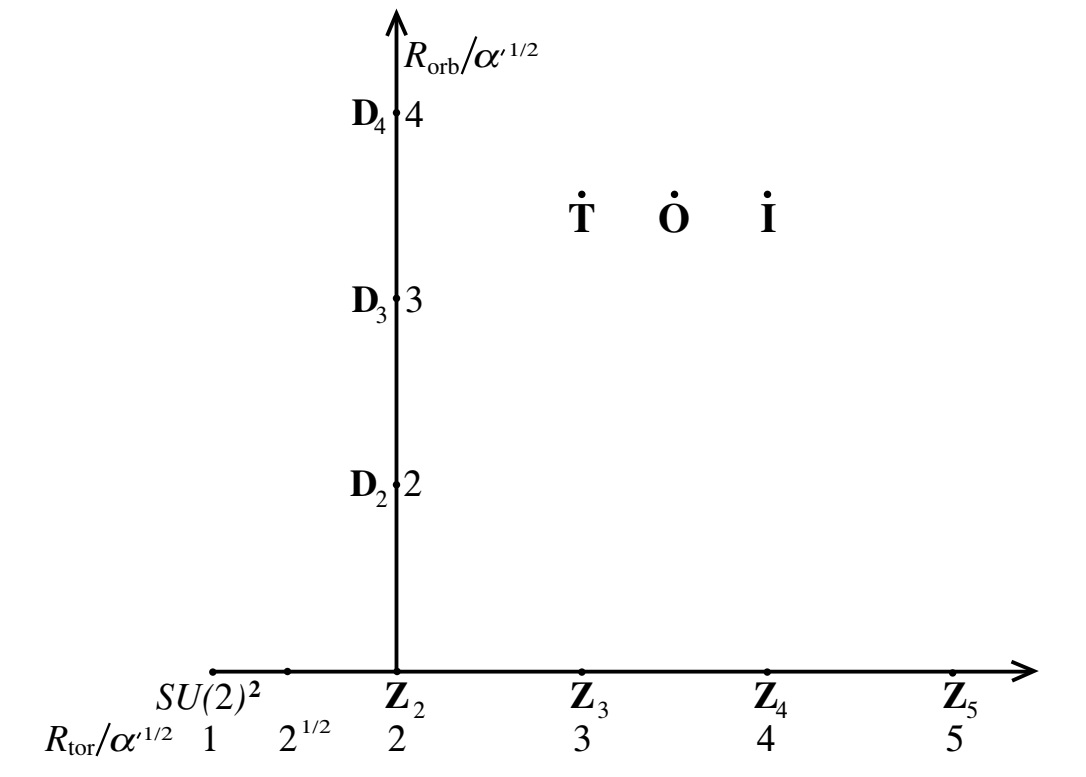
\includegraphics[width=0.8\textwidth,natwidth=814.5,natheight=582.75]{Fig8.2.jpg}
		\caption{$c=1$ CFT 的模空间. 水平轴是环向分支, 而垂直轴是轨形分支. 图中标出的点是用$SU(2)$群的一个离散子群扭曲获得的, 
		包含三个从四面体群, 八面体群和二十面体群获得的三个孤立点. 其它特殊半径, 诸如$R=(2 \alpha^{\prime})^{1/2}$处的环面, 后面会出现.}\label{Fig8.2}
	\end{center}
\end{figure}

这种等价性仅在这些半径处成立. 例如, 对于一般的$R$, 环向理论只有 $U(1) \times U(1)$规范对称性, 而轨形没有规范对称性. 
因此, 二者模空间的联系如图\ref{Fig8.2}所示. 有不同分支的模空间在特殊的点处会合, 在超对称理论中, 这一结构拥有非常普遍且重要的特征. 
一般而言, 在每一个分支会有不同的低能有效理论, 在这里的表现是低能规范对称性. 在特殊点的附近存在更多的轻场. 
随着我们沿着不同分支远离特殊点, 它们的不同子集会变得有质量.

环向分支与轨形分支交叉点附近的低能物理很有启发意义. 用\eqref{8.5.20}中的$r^{\prime}$扭曲的 $S U(2)$ 理论来描述它. 
在这一扭曲下留存的无质量标量是 $j^{3} \tilde{\jmath}^{3}$ 以及 $j^{i} \tilde{\jmath}^{j}$, 其中$i, j \in\{1,2\}$. 
既然它们是非扭的, 势与扭曲之前相同, 即 $\mathrm{det} M$. 标量场 $M_{i j}$依旧可以通过 $U(1) \times U(1)$ 旋转对角化, 
并且仅当一个对角元非零时, 势是平坦的. 然而, 现在模 $M_{33}$ 无法旋转至 $M_{11}$ 或 $M_{22}$, 所以这些方向在物理上不同. 
模$M_{33}$保持 $U(1) \times U(1)$ 不破坏, 并对应于沿着环向分支的移动. 模$M_{11}$ 或 $M_{22}$破缺了规范对称, 并对应于沿着轨形分支的移动. 
既然这个模是带荷的, 它的符号反转是规范变换, 所以物理上不同的轨形终于分支的交叉点. 我们无法同时变换两个模, 因为它们的线性组合不是平坦方向. 
轨形上的弦理论等价于圆上的弦理论, 这是相当可观的. 这表明弦看待时空几何的方式与我们并非完全相同.

沿着环向分支进行移动, 在 $SU(2)$半径的整数倍 $R=k \alpha^{\prime 1/2} $ 会有额外的无质量态. 这些态有 $(n, w)=(\pm 2 k, 0)$. 
我们可以认为这些点是这样获得的, 在$T$-对偶处理下,  $R=\alpha^{\prime 1/2} / k$,
 它们又是通过用$\mathds{Z}_{k}$对称性扭曲 $S U(2) \times S U(2)$理论得到
\begin{equation}
	X^{25} \rightarrow X^{25}+\frac{2 \pi \alpha^{\prime 1/2}}{k} \:. \label{8.5.22}
\end{equation}
这给 $j^{1}+\mi j^{2}$ 和 $\tilde{\jmath}^{1}+\mi \tilde{\jmath}^{2}$ 乘上了 $\exp (2 \pi \mi / k)$ , 因而幸存的无质量标量是
\begin{equation}
	j^{3} \tilde{\jmath}^{3}, \quad j^{1} \tilde{\jmath}^{1}+j^{2} \tilde{\jmath}^{2}, \quad 
	j^{1} \tilde{\jmath}^{2}-j^{2} \tilde{\jmath}^{1} \:. \label{8.5.23}
\end{equation}
这些中的第一个改变了环面的半径, 因而总是平坦方向. 然而, 因为在方向$M_{11}=M_{22}$ 或 $M_{12}=-M_{21}$上不会遇到势的平坦性条件\eqref{8.3.23}, 
从这些点中不再浮现其他分支.

偏移 \eqref{8.5.22} 生成了$S U(2) \times S U(2) $的$\mathds{Z}_{k}$子群. 我们来考察其他子群的扭曲. 
二面体群$\mathbf{D}_{k}$ 由偏移 \eqref{8.5.22} 和反射 $X^{25} \rightarrow-X^{25}$ 构成, 这给出了半径$k \alpha^{\prime 1/2}$处的轨形. 
其他三个离散子群是四面体群、八面体群以及二十面体群. 它们从CFT中移除了所有模, 所以扭曲CFT是孤立点, 不是连续族中的成员. 
不像 $\mathds{Z}_{k}$ 和 $\mathbf{D}_{k}$ 扭曲, 它们可以在所有半径处定义, 而这些包含 $S U(2)$元素的离散子群仅在离散半径处存在, 
因而半径不能在扭曲后变化. 有这种紧致化空间的弦论只会有一个标量——伸缩子. 

这是所有已知的 $c=1$的 CFT, 因而给出了所有已知的25维玻色弦背景.


\section{开弦} \label{sec:8.6}%{8.6 Open strings}

在开弦的环向紧致化中有一个新特征, 即有可能存在非平庸的威尔逊线, 规范场的平坦背景. 首先研究一些带有带荷场的$U(1)$规范理论, 考察常背景
\begin{equation}
	A_{25}(x^{M})=-\frac{\theta}{2 \pi R}=-\mi \Lambda^{-1} \frac{\partial \Lambda}{\partial x^{25}}, \quad 
	\Lambda(x^{25})=\exp \biggl(-\frac{\mi \theta x^{25}}{2 \pi R}\biggr) \:, \label{8.6.1}
\end{equation}
其中$\theta$是常数. 定域上看, 这是纯规范, 场强为零, 场方程是平庸的. 然而, 规范参量 $\Lambda$ 不满足时空周期性, 所以背景有物理效应. 
衡量这一效应的规范不变量是威尔逊线
\begin{equation}
	W_{q}=\exp \biggl(\mi q \oint \dif x^{25}\: A_{25}\biggr)=\exp (-\mi q \theta) \:. \label{8.6.2}
\end{equation}

首先考察电荷为$q$的点粒子, 它的规范固定作用量
\begin{equation}
	S=\int \dif \tau \: \biggl(\frac{1}{2} \dot{X}^{M} \dot{X}_{M}+\frac{m^{2}}{2}-\mi q A_{M} \dot{X}^{M}\biggr) \:. \label{8.6.3}
\end{equation}
规范作用量就是$-\mi q \int \dif x^{M}\, A_{M}$, 所以绕紧致维度一周的路径会挑出等于威尔逊线 $W_{q} $的相位. 正则动量是
\begin{equation}
	p_{25}=-\frac{\partial L}{\partial v^{25}}=v^{25}-\frac{q \theta}{2 \pi R} \:, \label{8.6.4}
\end{equation}
其中, 同\eqref{8.4.6}一样, $v^{25}=\mi \dot{X}^{25}$. 波函数在紧致维度中必须是周期的, 所以 $p_{25}=l/R$, $l$为整数, 并且
\begin{equation}
	v_{25}=\frac{2 \pi l+q \theta}{2 \pi R} \:. \label{8.6.5}
\end{equation}
湮灭物理态的哈密顿量是
\begin{equation}
	H=\frac{1}{2} (p_{\mu} p^{\mu}+v_{25}^{2}+m^{2}) \:, \label{8.6.6}
\end{equation}
由于 $v_{25}$ 依赖$\theta$, 所以 $-p_{\mu} p^{\mu}$ 发生了偏移. 相同的频谱可以在场描述下获得. 
注意, $v_{25}$ 正是规范不变动量$-\mi \partial_{25}-q A_{25}$.

我们也可做规范变换 $\Lambda^{-1}$令 $A_{25}$为零, 这一规范下带荷场不再是周期的, 
在$x^{25} \rightarrow x^{25}+2 \pi R$下挑出相位 $\exp (\mi q \theta)$. 物理量依旧是周期的. 正则动量现在偏移了, 我们有
\begin{equation}
	v_{25}=p_{25}=\frac{2 \pi l+q \theta}{2 \pi R}\:, \label{8.6.7}
\end{equation}
与之前一样, 对于规范不变动量 $v_{25}$获得了相同结果.

现在我们回到弦, 引入 $U(n)$ Chan-Paton 因子. 一般常数 $A_{25}$可以通过规范变换对角化
\begin{equation}
	A_{25}=-\frac{1}{2 \pi R} \operatorname{diag}(\theta_{1}, \theta_{2}, \ldots, \theta_{n}) \:. \label{8.6.8}
\end{equation}
这个规范场处在$U(n)$的对角群中, 即$U(1)^{n}$. 规范场与一般态的Chan-Paton因子的耦合为 $[A_{M}, \lambda]$, 
所以Chan-Paton 态 $|i j\rangle$ 中的弦在$U(1)_{i}$下有荷$+1$, 在$U(1)_{j}$下有荷$-1$, 在其他情况下为中性. 因此它有
\begin{equation}
	v_{25}=\frac{2 \pi l-\theta_{j}+\theta_{i}}{2 \pi R} \:. \label{8.6.9}
\end{equation}
那么开弦频谱就是
\begin{equation}
	m^{2}=\frac{(2 \pi l-\theta_{j}+\theta_{i})^{2}}{4 \pi^{2} R^{2}}+\frac{1}{\alpha^{\prime}}(N-1) \:. \label{8.6.10}
\end{equation}

考察规范玻色子, 这是 $l=0$ 且 $N=1$, 因此
\begin{equation}
	m^{2}=\frac{(\theta_{j}-\theta_{i})^{2}}{4 \pi^{2} R^{2}} \:. \label{8.6.11}
\end{equation}
在一般背景下, 所有 $\theta$都不同, 仅有的无质量矢量是对角的, $i=j$. 在这一情况下, 未破缺规范群是 $U(1)^{n} $. 
如果 $r$个 $\theta$ 相等, 相应的矢量的 $r \times r$矩阵是无质量的, 携带规范对称性$U(r)$. 将 $n$个 $\theta$分到集合 $r_{i}$中, 规范对称性是
\begin{equation}
	U(r_{1}) \times \ldots \times U(r_{s}), \quad \sum_{i=1}^{s} r_{i}=n \:. \label{8.6.12}
\end{equation}
像之前一样, 这有一个低能解释. 规范场$A_{25}$是 $U(n)$伴随表示中的25维标量, 而它的真空期望值将对称性破缺至$U(r_{1}) \times \ldots \times U(r_{s})$.

读者可以填补低能有效作用量的细节. 需要注意的是, 若紧致维度有$k$个, 势中会包含
\begin{equation}
	\operatorname{Tr}\Bigl([A_{m}, A_{n}]^{2}\Bigr) \:, \label{8.6.13}
\end{equation}
它来自26维Yang-Mills作用量中的场强. 这迫使不同方向的规范场在静态解中对易, 使得它们可同时对角化. 规范场中会给出$kn$个模, 
度规和反对称张量会给出 $k^{2}$ 个模.

\subsection*{$T$-对偶}

现在考察开弦频谱的 $R \rightarrow 0$ 极限. 若开弦的边界是 Neumann 边界, 它没有类似于 $w$ 的量子数; 它们总可以从紧致维上解开. 
所以, 当 $R \rightarrow 0$ 时, 动量不为零的态获得无限大质量, 但不再有新的连续态. 这与场论中的行为一致: 相应的态在25个时空维中移动.

我们知道有开弦的理论必有闭弦, 这貌似会产生矛盾. 这使得在 $R \rightarrow 0$的极限下, 闭弦在26个时空维中移动, 而开弦在25个时空维中移动. 
由此可推理出发生了如下事情: 开弦的内部与闭弦相同, 由同一“物质”构成, 所以依旧在26维振动. 区分开弦的正是它们的端点, 
所以它们必须限制在一个25维超平面上. 

事实确实如此, 我们可以用新的嵌入坐标来描述$T$-对偶理论
\begin{equation}
	X^{\prime 25}(z, \bar{z})=X_{L}^{25}(z)-X_{R}^{25}(\bar{z}) \:. \label{8.6.14}
\end{equation}
那么
\begin{equation}
	\partial_{n} X^{25}=-\mi \partial_{t} X^{\prime 25} \:, \label{8.6.15}
\end{equation}
其中 $n$是边界的法向,  $t$是边界的切向. 原始坐标上的 Neumann 边界就是对偶坐标上的 Dirichlet 边界: 每个弦端点的$X^{\prime 25}$坐标是固定的. 

我们先来考察没有威尔逊线的紧致化. 那么所有端点都约束在同一超平面上. 为看到这一点, 积分
\begin{align}
		X^{\prime 25}(\pi)-X^{\prime 25}(0) &= \int_{0}^{\pi} \dif \sigma^{1}\: \partial_{1} X^{\prime 25}
											 = -\mi \int_{0}^{\pi} \dif \sigma^{1}\: \partial_{2} X^{25} \nonumber \\
											&= -2 \pi \alpha^{\prime} v^{25}
											 = -\frac{2 \pi \alpha^{\prime} l}{R}=-2 \pi l R^{\prime} \:. \label{8.6.16}
\end{align}
$X^{\prime 25}$在两个端点之间的总变化是对偶维周期$2 \pi R^{\prime}$的整数倍, 所以末端处在周期$T$对偶空间的同一超平面上. 
对于两个不同的开弦, 它们之间交换引力子会给出连通世界面. 我们可以对此进行与\eqref{8.6.16}相同的讨论, 所以, 所有弦的端点都处在同一超平面上, 
见图\ref{Fig8.3}. 端点在其他24维依旧是随意移动的.

\begin{figure}[h]
	\begin{center}
		%width=0.8\textwidth,bb=0 0 761 723
		%1px=0.75pt
		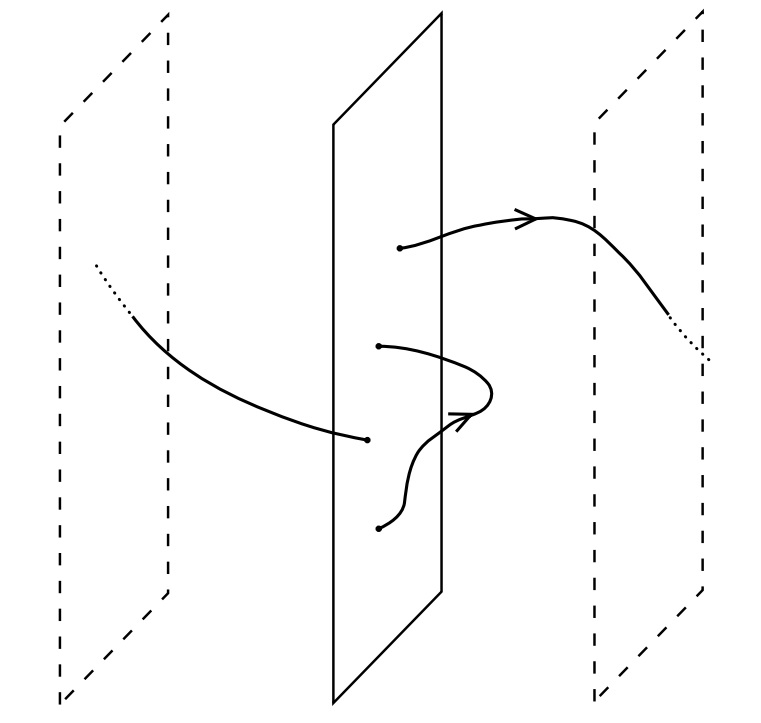
\includegraphics[width=0.7\textwidth,natwidth=532.7,natheight=530]{Fig8.3.jpg}
		\caption{端点连在超平面上的开弦. 虚线标出的平面是周期等价的平面. 图中展示出了两条弦, 缠绕数分别为1和0.}\label{Fig8.3}
	\end{center}
\end{figure}

现在我们来看威尔逊线的效应. 由于$v_{25}$中有偏移\eqref{8.6.9}, \eqref{8.6.16}被换成
\begin{equation}
	\Delta X^{\prime 25}=X^{\prime 25}(\pi)-X^{\prime 25}(0)=-(2 \pi l-\theta_{j}+\theta_{i}) R^{\prime} \:. \label{8.6.17}
\end{equation}
换句话说, 除去一个额外的归一化,  $i$ 态上的端点处在
\begin{equation}
	X^{\prime 25}=\theta_{i} R^{\prime}=-2 \pi \alpha^{\prime} A_{25, i i} \:. \label{8.6.18}
\end{equation}
因此, 一般会有$n$个不同的超平面, 见图\ref{Fig8.4}.

\begin{figure}[h!]
	\begin{center}
		%width=0.8\textwidth,bb=0 0 938 756
		%1px=0.75pt
		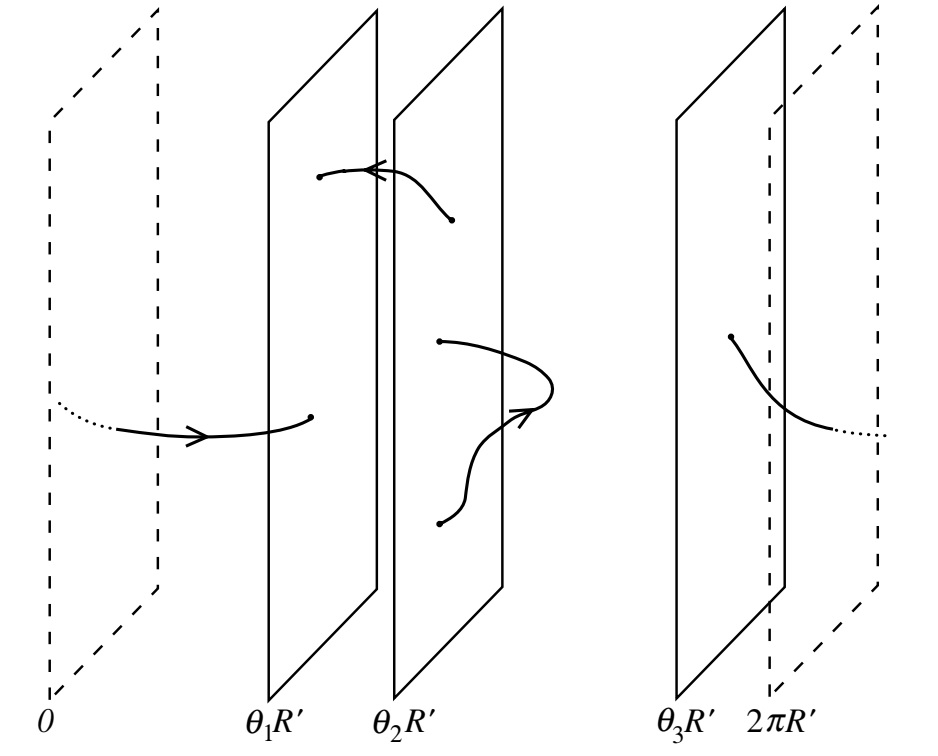
\includegraphics[width=0.8\textwidth,natwidth=656.6,natheight=555]{Fig8.4.jpg}
		\caption{处在不同位置的$n=3$个超平面, 上面连上了不同的弦. 忽略快子, 两端连在同一超平面的最轻弦是无质量的, 而连接两个不重合的超平面的弦由于张力是有质量的. 当两个超平面重合时, 连接超平面的最轻弦变成无质量的.}\label{Fig8.4}
	\end{center}
\end{figure}

我们来考察Chan-Paton态 $|i j\rangle$的模式展开, 并假定它在紧致维数上缠绕了$l$次
\begin{align}
	X^{\prime 25}(z, \bar{z}) &= \theta_{i} R^{\prime} - \frac{\mi R^{\prime}}{2 \pi}(2 \pi l-\theta_{j}+\theta_{i}) 
	\ln (z / \bar{z}) + \mi \biggl(\frac{\alpha^{\prime}}{2}\biggr)^{1/2} 
	\sum_{\substack{m=-\infty  \\  m \neq 0}}^{\infty} \frac{\alpha_{m}^{25}}{m}(z^{-m}-\bar{z}^{-m})  \nonumber \\
	&=\theta_{i} R^{\prime} + \frac{\sigma^{1}}{\pi} \Delta X^{\prime 25} - (2 \alpha^{\prime})^{1/2} 
	\sum_{\substack{m=-\infty  \\  m \neq 0}}^{\infty} \frac{\alpha_{m}^{25}}{m} \exp (-m \sigma^{2}) \sin m \sigma^{1} \:. \label{8.6.19}
\end{align}
频谱 \eqref{8.6.10} 变成
\begin{equation}
	m^{2}=\biggl(\frac{\Delta X^{\prime 25}}{2 \pi \alpha^{\prime}}\biggr)^{2}+\frac{1}{\alpha^{\prime}}(N-1) \:, \label{8.6.20}
\end{equation}
其中 $\Delta X^{\prime 25}$由\eqref{8.6.17}给定. 它是弦在给定分区中的最短长度.

现在来考察, 如果有多个紧致维, 这个图景怎么推广. 设 $X^{m}$是周期维, 其中 $p+1 \leq m \leq 25$. 我们将周期维写成对偶坐标的形式. 
$X^{m}$上的 Neumann 条件又一次变成对偶坐标 $X^{\prime m}$上的 Dirichlet 条件, 所以开弦端点拘束在$n$ 个平行的$(p+1)$-维子空间中. 
对于每个子空间, 不同方向的威尔逊线变成独立坐标.

由于平移不变性被开弦边界条件破坏了, 对偶背景相当古怪. 这反映了如下事实: 在原始开弦理论中, 缠绕数不守恒, 而缠绕数$T$对偶到动量. 
$T$对偶只是同一理论的不同描述. 更进一步, 当紧致半径很小时, 那么就应该自然地使用$T$对偶图景.

\section{D膜}%{8.7 D-branes}
我们现在知道, 当开弦理论紧致化在一个小环面上时, 它的物理可以描述成在大环面上的紧致化, 但是开弦的端点约束在子空间中. 事实上, 这些子空间本身是新的动力学客体.

在一般构形下考虑无质量开弦的频谱, 在这种构形下, 所有$\theta_{i}$都不同, 简单起见, 只取一个坐标是对偶化的. 
忽视快子, 质量\eqref{8.6.20}仅在$N=1$且 $\Delta X^{\prime 25}=0 $ 时为零. 即, 两个端点处在同一超平面且缠绕数为零. 因而我们有无质量态
\begin{subequations} \label{8.7.1}
\begin{align}
	&\alpha_{-1}^{\mu}|k; ii\rangle \:, \quad \mathscr{V} = \mi \partial_{t} X^{\mu}  \:, \label{8.7.1a} \\
	&\alpha_{-1}^{25} |k; ii\rangle \:, \quad \mathscr{V} = \mi \partial_{t} X^{25} = \partial_{n} X^{\prime 25} \:. \label{8.7.1b}
\end{align}
\end{subequations}
它们显然就是原始理论中的无质量态, $T$-对偶只是给了同一频谱的不同图景. 对于一般的威尔逊线, 唯一的无质量开弦态将是$n$个无质量$U(1)$矢量. 
在\eqref{8.7.1}中, 我们根据它们是切于超平面还是垂直于超平面将其分类. 有切向极化的25个态构成了处在超平面上的规范场, 
而它在$T$-对偶理论中有一个简单且重要的解释: 它是超平面形状的坐标集. 从常数规范场\eqref{8.6.18}对应于超平面的均匀平移就可以看到这一点. 
依赖$x^{\mu}$的背景可以转至一个依赖$x^{\mu}$的平移, 一个弯曲的超平面, 而场 $A_{ii}^{25}$ 的量子对应超平面的微小振荡.

这与时空上发生的现象相同. 我们从平坦背景中的弦出发, 发现无质量闭弦态对应几何的涨落. 
在这里, 我们首先发现超平面, 然后发现特定的开弦态对应于超平面的涨落. 我们不应该对超平面有动力学感到惊讶. 
弦论包含引力. 引力波穿越超平面时将会扰动时空本身, 所以超平面很难保持刚性.

因此, 超平面确实是动力学客体, 这是D膜. 对于$25-p$个维度做对偶会得到p维膜, 称为 D$p$-膜. 
利用这个术语, 原始的 $U(n)$ 开弦理论会包含 $n$个 D25-膜. D25-膜填满了空间, 所以弦端点没有约束: 它仅对应一般的 Chan-Paton 因子.

既然$T$ 对偶交换了Neumann与Dirichlet边界条件, 在与D$p$膜相切的方向上做$T$对偶会将其约化至 D$(p{-}1)$-膜, 
而在垂直方向上做 $T$ 对偶则将其约化至D$(p{+}1)$-膜. 非平庸角的情况也会立刻出现. 

我们本可以通过研究Dirichlet边界本身出发. 这里我们所采取的路线是从$T$对偶发现它们, 这一方法能更好的发展它们的性质. 
也可证明, 通过一个连续的过程, 我们能从``普通''态到达包含D-膜的态. 即, 取普通理论的$R \rightarrow 0$极限, 这使得非紧致空间中有$n$个D-膜. 
在超弦中, 我们将用这一点来论证D-膜是理论的非微扰定义中的重要部分. 对于玻色弦, 由于没有很强的证据表明它有非微扰定义, 我们不做这个讨论. 
玻色弦论有可能仅是作为超弦的部分而存在.

我们来看一下$T$对偶图景中的$U(n)$对称性破缺. 当没有D-膜重合时, 仅在每个D-膜上有无质量矢量, 这给出规范群 $U(1)^{n}$. 
如果有$r$个D-膜重合, 那么会有额外的无质量态, 连接这些膜的弦长为零: 当$n=0$时, 若 $i$ 与$j$均在集合$r$中, 
质量公式\eqref{8.6.20}中的 $\Delta X^{\prime 25}$为零. 因此, 存在$r^{2}$ 个矢量, 构成$U(r)$规范群的伴随表示. 
这与对偶威尔逊线图景中发现的相同. 然而, 令人惊奇的是, 在垂直D-膜的方向上会有$r^{2}$个无质量标量. 我们会在下面讨论它的意义.

\subsection*{D-膜作用量}
在D$p$-膜的世界体上, 无质量场是$U(1)$矢量和描述涨落的 $25{-}p$ 世界膜标量. 这个系统的低能有效作用量总是值得考察的. 
我们取对偶半径$R^{\prime}$为无穷, 只考虑相应26维时空中的单个D膜. 世界膜场与无质量闭弦场有相互作用, 而它的作用量在\ref{sec:3.7}节讨论过. 
引入膜上的坐标 $\xi^{a}$, 其中$a=0, \ldots p$. 膜上的场是嵌入 $X^{\mu}(\xi)$ 以及规范场$A_{a}(\xi)$. 我们声明作用量
\begin{equation}
	\bm{S}_{p} = -T_{p} \int \dif^{p+1} \xi \: 
				\me^{-\Phi}[-\operatorname{det}(G_{ab} + B_{ab} + 2 \pi \alpha^{\prime} F_{a b})]^{1/2} \:, \label{8.7.2}
\end{equation}
其中$T_{p}$是待定常数. 这里
\begin{equation}
	G_{ab}(\xi) = \frac{\partial X^{\mu}}{\partial \xi^{a}} \frac{\partial X^{\nu}}{\partial \xi^{b}} G_{\mu \nu}(X(\xi)), \quad 
	B_{ab}(\xi) = \frac{\partial X^{\mu}}{\partial \xi^{a}} \frac{\partial X^{\nu}}{\partial \xi^{b}} B_{\mu \nu}(X(\xi)) \label{8.7.3}
\end{equation}
是膜上的诱导度规以及诱导反对称张量.

基于一般推理就可以理解\eqref{8.7.2}的所有特征. 首先, 只考察时空度规以及嵌入, 
最简单且导数最少的坐标无关作用量是 $(-\operatorname{det} G_{a b})^{1/2}$的积分, 即世界体积. 
注意到, 这一项经由诱导场\eqref{8.7.3}对$X^{\mu}(\xi)$有隐式关系. 围绕一个平坦D-膜做展开, 这给出涨落的作用量, 
就像Nambu-Goto作用量作用量描述了弦的涨落.

出现对伸缩子的依赖 $\me^{-\Phi} \propto g_{\mathrm{c}}^{-1}$ 是因为这是开弦树图作用量. 
开弦场的自相互作用, 以及它们与闭弦场的耦合, 最初来自于圆盘.

对 $F_{ab}$ 的依赖性可以通过$T$-对偶理解. 考察沿 $X^{1}$ 和 $X^{2}$ 方向铺展的D膜, 其他方向未指定, 并令上面有一个常数规范场 $F_{12}$. 
去往规范 $A_{2}=X^{1} F_{12}$. 现在沿$X^{2}$方向取$T$-对偶. 在这一方向的Neumann条件就变成了Dirichlet条件, 所以, D膜少了一个维数. 
然而, 势与坐标之间的关系\eqref{8.6.18}暗示了D-膜在 (1-2)-平面中是倾斜的
\begin{equation}
	X^{\prime 2}=-2 \pi \alpha^{\prime} X^{1} F_{12} \:. \label{8.7.4}
\end{equation}
这个倾斜赋予了作用量一个几何因子
\begin{equation}
	 \int \dif X^{1}\: \Bigl[1 + (\partial_{1} X^{\prime 2})^{2}\Bigr]^{1/2} 
	=\int \dif X^{1}\: \Bigl[1 + (2 \pi \alpha^{\prime} F_{12})^{2}\Bigr]^{1/2} \:. \label{8.7.5}
\end{equation}
对任意D-膜, 通过推动使其与坐标轴对齐, 并进行旋转, 使 $F_{ab}$ 变成对角形式, 可以将作用量约化至每一平面中的因子\eqref{8.7.5}的积, 
等价于行列式中的 $F_{ab}$ 项. 规范场构成的行列式称为Born-Infeld作用量, 它最初是为了解决量子电动力学的短程发散问题.

最后, 对 $B_{ab}$ 的依赖关系由如下讨论给出. 在弦的世界面作用量中, 闭弦场$B_{\mu \nu}$与开弦场$A^{\mu}$以如下形式出现
\footnote{对于熟悉微分形式的读者, 这是
	\[ \frac{\mi}{2 \pi \alpha^{\prime}} \int_{M} B + \mi \int_{\partial M} A \:. \]
后面的方程可以用类似的方式翻译.}
\begin{equation}
	\frac{\mi}{4 \pi \alpha^{\prime}} \int_{M} \dif^{2} \sigma \: g^{1/2} \epsilon^{ab} \partial_{a} X^{\mu} \partial_{b} X^{\nu} 
	B_{\mu\nu} + \mi \int_{\partial M} \dif X^{\mu} \:A_{\mu} \:. \label{8.7.6}
\end{equation}
这些场中的每一个都会附带一个时空规范不变性, 为了与时空理论相容必须予以保留. 通常的规范变换
\begin{equation}
	\delta A_{\mu}=\partial_{\mu} \lambda \label{8.7.7}
\end{equation}
是作用量\eqref{8.7.6}的一个不变性, 边界项会差一个全导数的积分. 反对称张量变分
\begin{equation}
	\delta B_{\mu \nu} = \partial_{\mu} \zeta_{\nu} - \partial_{\nu} \zeta_{\mu} \label{8.7.8}
\end{equation}
会使得``块''作用量差一个全导数, 但在有边界的世界面上, 这给出表面项. 要使得它抵消, 在张量规范对称性, 开弦场 $A_{\mu}$ 要有变换
\begin{equation}
	\delta A_{\mu}=-\zeta_{\mu} / 2 \pi \alpha^{\prime} \:. \label{8.7.9}
\end{equation}
现在, 只有组合
\begin{equation}
	B_{\mu \nu}+2 \pi \alpha^{\prime} F_{\mu \nu} \equiv 2 \pi \alpha^{\prime} \mathscr{F}_{\mu \nu}  \label{8.7.10}
\end{equation}
在两个对称性下是不变的, 因此出现在作用量中的必须是这个组合. 因此, 作用量的形式\eqref{8.7.2}就完全确定了.

作为检验, 由于相同的组合出现在共形规范下的世界面作用量中, 很自然地, 组合 $G_{\mu \nu}+B_{\mu \nu}$ 应该出现. 
也可以取各种开弦振幅以及开弦-闭弦振幅的低能极限来决定作用量\eqref{8.7.2}, 但这会费劲得多.

对于$n$个分立的D-膜, 作用量是$n$份儿单个D-膜作用量. 然而, 我们已经看到, 当D-膜重合时, 膜上会有 $n^{2}$ 个, 而不是 $n$个无质量矢量和标量, 
我们将写下这一情况的有效作用量. 场 $X^{\mu}(\xi)$以及 $A_{a}(\xi)$ 现在将是 $n \times n$ 矩阵. 对于规范场, 
含义是显然的——它变成了非阿贝尔 $U(n)$ 规范场. 然而, 对于坐标集 $X^{\mu}$, 含义是不清楚的: $n$ 个D-膜到时空的嵌入坐标集扩展成 $n \times n$ 矩阵. 
已经证明, 非对易几何在D-膜的动力学中扮演了重要角色, 这里有一个猜想: 它是时空特性的一个重要线索.

通过考察有效作用量, 我们可以获得更多启发. 作用量中现在有了非导数项, 它是坐标集的势, 这可以从常数 $A_{m}$ 场的 $T$-对偶中推断出来. 
对于这样的矢量势, 场强就是$[A_{m}, A_{n}]$, 它在$T$-对偶图景中变成了$(2 \pi \alpha^{\prime})^{-2}[X_{m}, X_{n}]$. 
在场强中展开, 作用量的领头阶大约是
\begin{equation}
	V \propto \operatorname{Tr}([X_{m}, X_{n}][X^{m}, X^{n}]) \:. \label{8.7.11}
\end{equation}
这个势在$X^{m}=0$处的二阶导数为零, 这使得所有$k n^{2}$个标量均无质量; 同以往一样 $k=25{-}p$ 是对偶维数. 
然而平坦维数的空间更小些. 势是平方和, 所以只在所有 $[X^{m}, X^{n}]$为零时为零. 我们可以用 $U(n)$对称性去往 $X^{m}$ 都对角的规范. 
因此会有 $kn$ 个平坦方向, 正是对角元个数. 这样, $kn$ 个对角元可以解释成 $n$ 个D$p$-膜坐标集. 
因此\eqref{8.7.11}正确地介入了分离D-膜与重合D-膜的物理.

当 $X^{m}$ 对易时, 作用量应该退化到$n$个分立的D-膜, 所以有
\begin{align}
	\bm{S}_{p} &= -T_{p} \int \dif^{p+1} \xi \: \operatorname{Tr} \Bigl\{ \me^{-\Phi}
	              [-\operatorname{det}(G_{ab} + B_{ab} + 2 \pi \alpha^{\prime} F_{ab})]^{1/2} \nonumber \\
		       &\qquad \qquad \qquad \quad + O([X^{m}, X^{n}]^{2})\Bigr\} \:. \label{8.7.12}
\end{align}
行列式取在世界体指标 $ab$上, 迹取在 $n$个 Chan-Paton指标上. 迹是合适的 $U(n)$ 不变量, 对于对角矩阵, 它退化成对分离D-膜的求和. 
对对易子的完整依赖关系要比简单的势 \eqref{8.7.11} 复杂得多, 其中会包含与其他场的耦合, 以及对易子的高阶修正. 
然而, 关键性质, 平坦方向的形式是不受影响的. 通过从完全Neumann情况下的 Born-Infeld 作用量出发, 并进行$T$-对偶, 我们可得到完全的依赖性. 
附带地, 包含场强对易子的高阶导数项不能仅用 $T$ 对偶就决定下来.

\subsection*{D-膜张力}
计算常数$T_{p}$是很有意义的, 并且对于超弦, 它的精确值非常重要. 在进行显式的计算之前, 注意到从$T$对偶可得到 $T_{p}$ 的递推关系. 
注意到, 在常数伸缩子背景下, D$p$-膜的张力是 $T_{p} \me^{-\Phi}$: 这是静态D$p$-膜单位体积内作用量的相反数. 
现在考察这样的D$p$-膜, 与该D$p$膜相切的 $p$ 个方向周期等价. 即, D$p$-膜绕在时空中的一个$p$-环面上. 它的质量是它的张力乘以它的环面的面积
\begin{equation}
	T_{p} \me^{-\Phi} \prod_{i=1}^{p}(2 \pi R_{i}) \:. \label{8.7.13}
\end{equation}
现在, 对其中一个周期方向$X^{p}$取$T$对偶. 这样不改变质量, 只是同样一个态的新描述. 用$T$-对偶理论的伸缩子\eqref{8.3.31}, 质量\eqref{8.7.13}是
\begin{equation}
	2 \pi \alpha^{\prime 1/2} T_{p} \me^{-\Phi^{\prime}} \prod_{i=1}^{p-1}(2 \pi R_{i}) \:. \label{8.7.14}
\end{equation}
\begin{tcolorbox}
	\begin{remark}
		利用了$\sqrt{\alpha^\prime}\me^{-\Phi^\prime}/R_p=\me^{-\Phi}$	
	\end{remark}	
\end{tcolorbox}
\noindent 然而, 在对偶理论中, 这相当于是 $\mathrm{D}(p{-}1)$-膜缠绕在$(p{-}1)$-环面上, 所以它的质量是
\begin{equation}
	T_{p-1} \me^{-\Phi^{\prime}} \prod_{i=1}^{p-1}(2 \pi R_{i}) \:. \label{8.7.15}
\end{equation}
联立 \eqref{8.7.14} 和 \eqref{8.7.15} 给出
\begin{equation}
	T_{p}=T_{p-1} / 2 \pi \alpha^{\prime 1/2} \:, \label{8.7.16}
\end{equation}
除了一个总的归一化外, 这完全决定了$T_{p}$.

为了决定D-膜张力的实际值, 我们需要计算弦振幅. 例如, 我们可以从D-膜的引力耦合将其推断出来, 这个振幅由一个带有引力子顶点算符的圆盘给出. 
然而, 这包含一个未知的比值 $g_{\mathrm{c}} / g_{\mathrm{o}}^{2}$, 闭弦耦合来自于顶点算符, 而开弦耦合源于圆盘. 
我们可以用另一方法获得绝对归一化. 考察两个平行的D$p$-膜, 它们分别在 $X_{1}^{m}=0$ 和 $X_{2}^{m}=y^{m}$ 处. 
通过交换闭弦, 这二者可以感到彼此的存在, 如图\ref{Fig8.5}所示. 弦振幅是圆环, 没有顶角算符, 可以用上一章的方法计算出来. 
那么, 交换引力子和伸缩子给出的极点, 就给出了闭弦态与D-膜的耦合$T_{p}$.
\begin{figure}
	\begin{center}
		%width=0.8\textwidth,bb=0 0 609 717
		%1px=0.75pt
		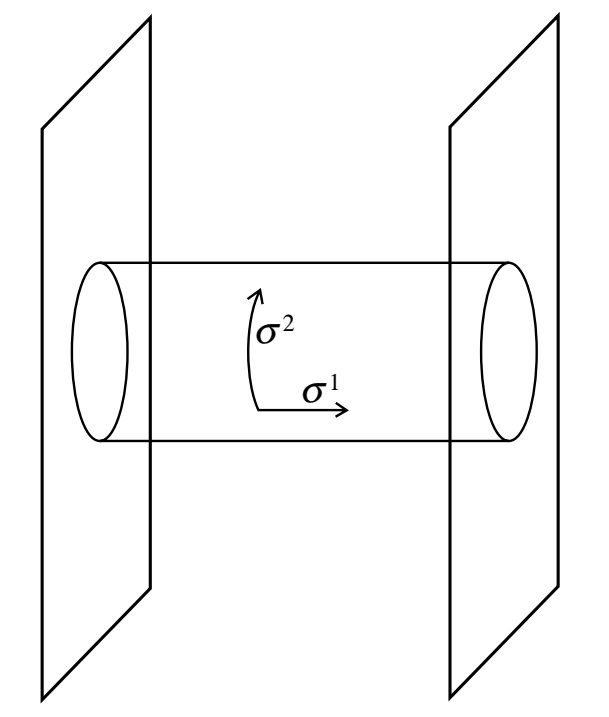
\includegraphics[width=0.6\textwidth,natwidth=426.3,natheight=520]{Fig8.5.jpg}\\
		\caption{在两个D-膜之间交换一个闭弦. 等价地, 这是端点连在两个D-膜的开弦的真空圈.}\label{Fig8.5}
	\end{center}
\end{figure}


在\ref{sec:7.4}节中, 我们用开弦圈计算了圆环真空振幅, 但从模积分的 $t \rightarrow 0$ 极限中发现了闭弦极点. 
这正是我们感兴趣的极点, 但计算振幅的最简单方法是视其为开弦圈. 事实上, 只要稍许改变, 就能用之前的结果\eqref{7.4.1}. 
动量积分的数目从26减少到$p{+}1$, 类似地, $V_{26}$ 变成 $V_{p+1}$; 权重 $h_{i}$ 由于拉伸开弦获得额外项 $y^{2} / 4\pi^{2} \alpha^{\prime}$; 
Chan-Paton 权重 $n^{2}$ 变成2(因为弦连接的方向有两个). 因此有
\begin{align}
	\mathscr{A} &= \mi V_{p+1} \int_{0}^{\infty} \frac{\dif t}{t} (8 \pi^{2} \alpha^{\prime} t)^{-(p+1)/2} 
				   \exp (-t y^{2} / 2 \pi \alpha^{\prime}) \eta(\mi t)^{-24}  \nonumber \\
				&= \frac{\mi V_{p+1}}{(8 \pi^{2} \alpha^{\prime})^{(p+1)/2}} 
				   \int_{0}^{\infty} \dif t\: t^{(21-p)/2} \exp (-t y^{2} / 2 \pi \alpha^{\prime}) \nonumber \\
				& \qquad \qquad \qquad \qquad \qquad  \times[\exp (2 \pi/t)+24+\cdots] \:, \label{8.7.17}
\end{align}
其中渐近展开以\ref{sec:7.4}节方法获得. 第一项是快子交换, 所以是玻色人工产物. 对第二项积分给出
\begin{align}
	\mathscr{A} &= \mi V_{p+1} \frac{24}{2^{12}}(4 \pi^{2} \alpha^{\prime})^{11-p} \pi^{(p-23)/2} 
				   \Gamma\biggl(\frac{23-p}{2}\biggr)|y|^{p-23}  \nonumber \\
				&= \mi V_{p+1} \frac{24 \pi}{2^{10}}(4 \pi^{2} \alpha^{\prime})^{11-p} G_{25-p}(y) \:, \label{8.7.18}
\end{align}
其中 $G_{d}(y)$ 是$d$ 维中无质量标量的格林函数, $-\nabla^{2}$的逆.

我们现在要与相同振幅的场论计算作一比较. 既然反对称张量不与D-膜耦合, 从时空作用量\eqref{3.7.25}中, 相关项是
\begin{equation}
	\bm{S}=\frac{1}{2 \kappa^{2}} \int \dif^{26} X \: (-\tilde{G})^{1/2} 
		   \biggl(\tilde{\bm{R}}-\frac{1}{6} \nabla_{\mu} \tilde{\Phi} \tilde{\nabla}^{\mu} \tilde{\Phi}\biggr) \:. \label{8.7.19}
\end{equation}
加波浪线是指爱因斯坦度规; 由于这一形式的作用量与伸缩子退耦, 所以比较方便. 加波浪线的伸缩子已经进行了偏移, 使得它的真空期望值为零. 
以同一变量的形式, D-膜作用量\eqref{8.7.2}中的相关项是
\begin{equation}
	\bm{S}_{p} = -\tau_{p} \int \dif^{p+1} \xi \: \exp \biggl(\frac{p-11}{12} \tilde{\Phi}\biggr)
				 (-\operatorname{det} \tilde{G}_{ab})^{1/2} \:. \label{8.7.20}
\end{equation}
我们定义了 $\tau_{p}=T_{p} \me^{-\Phi_{0}}$; 当伸缩子的背景值是$\Phi_{0}$时, 这是D$p$-膜的真实物理张力.

类比图\ref{Fig8.5}的场论图是在D-膜之间交换伸缩子或引力子. 为了获得传播子, 
我们将时空作用量展至$h_{\mu\nu}=\tilde{G}_{\mu\nu}-\eta_{\mu\nu}$ 和 $\tilde{\Phi}$的二阶. 
另外, 对于引力计算, 我们需要选择规范. 对于微扰计算, 最简单的规范是
\begin{equation}
	F_{\nu} \equiv \partial^{\hat{\mu}} h_{\mu \nu}-\frac{1}{2} \partial_{\nu} h^{\hat{\mu}}{}_{\mu}=0 \:, \label{8.7.21}
\end{equation}
其中, 加``帽子''是指用平坦度规 $\eta^{\mu \nu}$ 升降指标. 将作用量展开至二阶, 并加上规范固定项 $-F_{\nu} F^{\hat{\nu}} / 4\kappa^{2}$, 
时空作用量变成
\begin{equation}
	\bm{S}=-\frac{1}{8 \kappa^{2}} \int \dif^{26} X \: \biggl( \partial_{\mu} h_{\nu \lambda} 
	\partial^{\hat{\mu}} h^{\hat{\nu} \hat{\lambda}}-\frac{1}{2} \partial_{\mu} h^{\hat{\nu}}{}_{\nu} 
	\partial^{\hat{\mu}} h^{\hat{\lambda}}{}_{\lambda}+\frac{2}{3} \partial_{\mu} \tilde{\Phi} \partial^{\hat{\mu}} \tilde{\Phi}\biggr) \:. \label{8.7.22}
\end{equation}
观察动能项, 由此获得动量空间传播子
\begin{subequations} \label{8.7.23}
\begin{align}
		\langle\tilde{\Phi} \tilde{\Phi}\rangle &=-\frac{(D-2) \mi \kappa^{2}}{4 k^{2}}  \:, \label{8.7.23a} \\
		\langle h_{\mu \nu} h_{\sigma \rho}\rangle &=-\frac{2 \mi \kappa^{2}}{k^{2}}
		\biggl(\eta_{\mu \sigma} \eta_{\nu \rho}+\eta_{\mu \rho} \eta_{\nu \sigma}-\frac{2}{D-2} \eta_{\mu \nu} \eta_{\sigma \rho}\biggr) \:. \label{8.7.23b}
\end{align}
\end{subequations}
为了之后参考, 我们给出了一般的$D$. 围绕一般平坦构形展开, D-膜作用量是
\begin{equation}
	\bm{S}_{p}=-\tau_{p} \int \dif^{p+1} \xi \: \biggl(\frac{p-11}{12} \tilde{\Phi}-\frac{1}{2} h_{aa}\biggr) \:. \label{8.7.24}
\end{equation}
注意这里的$h_{\mu \nu}$ 仅对与D-膜相切的方向求迹; 我们已经取 $\xi$ 为度规为$\delta_{ab}$的直角坐标.

我们现在可读出费曼图
\begin{align}
	\mathscr{A} &= \frac{\mi \kappa^{2} \tau_{p}^{2}}{k_{\perp}^{2}} V_{p+1} 
				   \left\{6\left[\frac{p-11}{12}\right]^{2}+\frac{1}{2}\left[2(p+1)-\frac{1}{12}(p+1)^{2}\right]\right\} \nonumber \\
			    & =\frac{6 \mi \kappa^{2} \tau_{p}^{2}}{k_{\perp}^{2}} V_{p+1} \:. \label{8.7.25}
\end{align}
\begin{tcolorbox}
	\begin{remark}
		上式来自于$\langle S_p S_p \rangle$.
	\end{remark}	
\end{tcolorbox}
\noindent 与\eqref{8.7.18}比较给出
\begin{equation}
	\tau_{p}^{2} = \frac{\pi}{256 \kappa^{2}} (4 \pi^{2} \alpha^{\prime})^{11-p} \:. \label{8.7.26}
\end{equation}
这与$T$-对偶给出的递推关系一致.

作为一个应用, 考察有 $n$个25-膜的态, 这与普通的$n$值Chan-Paton 因子相同. 将25-膜作用量\eqref{8.7.12}展至规范场的二阶, 给出
\begin{equation}
	\frac{\tau_{25}}{4}(2 \pi \alpha^{\prime})^{2} \operatorname{Tr}(F_{\mu \nu} F^{\mu \nu}) \:. \label{8.7.27}
\end{equation}
这关联了开弦规范耦合与闭弦引力耦合. 利用\eqref{6.5.14}, \eqref{6.5.16}, \eqref{6.6.15}, 和 \eqref{6.6.18}, 
我们可以将其写为顶点算符归一化 $g_{\mathrm{c}}$ 与 $g_{\mathrm{o}}$之间的关系
\begin{equation}
	\frac{g_{\mathrm{o}}^{2}}{g_{\mathrm{c}}} = \frac{4 \pi \alpha^{\prime} g_{\mathrm{o}}^{\prime 2}}{\kappa}
											  = 2^{18} \pi^{25 / 2} \alpha^{\prime 6} \:. \label{8.7.28}
\end{equation}
它拥有正确的形式, 开弦耦合的平方正比于闭弦耦合, 但现在有了数值系数. 我们经由幺正性, 从圆环中分解出闭弦极点, 或参看习题7.9


\section{非定向弦的$T$-对偶} \label{sec:8.8}%{8.8 T-duality of unoriented theories}
在非定向的弦理论中,  $R \rightarrow 0$的极限也会给出有趣的新物理. 首先考察闭弦理论. 为了构成非定向理论, 我们在态上强加$\Omega=+1$. 
沿用\ref{sec:8.5}节的讨论, 我们也可认为这是规范化 $\Omega$. 特别地, 用来构建世界面的跃迁函数现在会反转方向, 并且这产生了非定向世界面.

$T$-对偶理论是通过用坐标$X^{\prime m}(z, \bar{z})= X_{L}^{m}(z)-X_{R}^{m}(\bar{z})$ 替换 
$X^{m}(z, \bar{z})=X_{L}^{m}(z)+X_{R}^{m}(\bar{z})$获得的. 在原始描述中, 我们规范化世界面宇称 $\Omega$, 它的作用
\begin{equation}
	\Omega: X_{L}^{M}(z) \leftrightarrow X_{R}^{M}(z) \:. \label{8.8.1}
\end{equation}
以$T$-对偶坐标, 这是
\begin{subequations} \label{8.8.2}
	\begin{align}
		\Omega: \quad X^{\prime m}(z, \bar{z})  &\leftrightarrow-X^{\prime m}(\bar{z}, z) \:, \label{8.8.2a} \\
		X^{\mu}(z, \bar{z})  &\leftrightarrow X^{\mu}(\bar{z}, z) \:, \label{8.8.2b}
	\end{align}
\end{subequations}
同之前一样,  $m$ 标记取$T$-对偶的坐标, $\mu$ 标记不取$T$-对偶的坐标. 在对偶图景中, 对称性\eqref{8.8.2}因此是世界面宇称变换和时空反演的乘积. 
我们看到规范化世界面宇称仅产生非定向理论, 而规范化反演仅产生轨形. 组合投射的结果称为\emph{定向形(orientifold)}.

定向形与轨形非常类似. 将弦的波函数分成它的内部以及依赖质心$x^{m}$的部分, 取内部波函数为 $\Omega$的本征态. 
那么到 $\Omega=+1$ 的投射就表明 $-x^{m}$处的弦波函数与 $x^{m}$处相同, 所差的仅是一个符号. 例如度规与反对称张量的分量满足
\begin{subequations} \label{8.8.3}
\begin{align}
		G_{\mu \nu}(x^{\prime}) &= G_{\mu \nu}(x) \:, \quad  B_{\mu \nu}(x^{\prime})=-B_{\mu \nu}(x) \:, \label{8.8.3a} \\ 	
		G_{\mu n}(x^{\prime}) & =-G_{\mu n}(x) \:, \quad  B_{\mu n}(x^{\prime})=B_{\mu n}(x) 	\:, \label{8.8.3b} \\
		G_{m n}(x^{\prime}) &= G_{m n}(x) \:, \quad  B_{m n}(x^{\prime})=-B_{m n}(x) \:, \label{8.8.3c}
\end{align}
\end{subequations}
其中 $(x^{\mu}, x^{m})^{\prime} = (x^{\mu},-x^{m})$.  对于每个 $m, n$ 会有一个负号, 对于 $B_{M N}$会有另一个负号; 这与轨形完全相同. 
换句话说, $T$-对偶时空是环面$T^{k}$模掉$k$个紧致维中的 $\mathds{Z}_{2}$ 反射, 与轨形的构建完全相同. 
例如, 如果只有一个周期性, 对偶时空是线段 $0 \leq x^{25} \leq \pi R^{\prime}$, 端点处是定向形固定平面.

注意到, 当远离定向形不动平面时, 定域物理是定向弦论的物理. 不像原始的非定向理论, 在那里投射定域地移除一半的态, 
在这里它将任意点的弦波函数与它在镜像点的值关联起来, 就像\eqref{8.8.3}中那样.

轨形构造与定向形构造的一个不同之处在于后者没有扭态的直接类比, 原因是Klein瓶没有模变换 $\tau \rightarrow -1/\tau$. 
考察图\ref{Fig8.6}, 它给出了环面与Klein瓶. 在环面上, 投射算符在图\ref{Fig8.6}a的类时方向上插入了一个扭转; 将这个图转$90^{\circ}$, 
这变成了空间方向上的扭转, 暗示了频谱中有扭态. 然而, 如果图\ref{Fig8.6}b的Klein瓶转了$90^{\circ}$, 相对边上的时间方向无法匹配. 
所以在这个道上没有中间态的解释. 由此要注意的是, 定向形平面不能是动力学的. 不像D-膜的情况, 没有弦模拴在定向形平面上来代表它的形状的涨落. 
我们的启发性讨论——引力波迫使D-膜在这里振荡, 并不适用于定向形平面. 最终, 等价关系 \eqref{8.8.3} 变成不动平面上的边界条件, 使得入射波与反射波抵消. 
对于D-膜, 反射波是弦耦合的高阶量.

\begin{figure}
	\begin{center}
		%width=0.8\textwidth,bb=0 0 1072 381
		%1px=0.75pt
		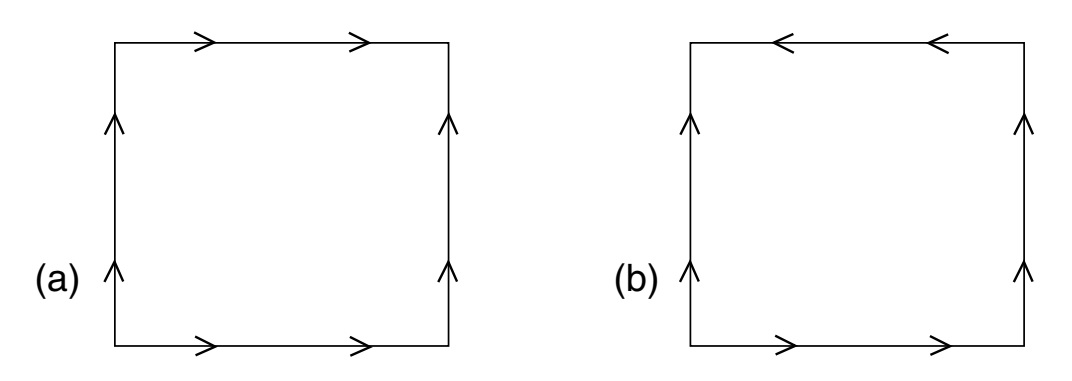
\includegraphics[width=0.8\textwidth,natwidth=750.4,natheight=266.7]{Fig8.6.jpg}
		\caption{粘合对边给出了(a)环面和(b) Klein瓶.}\label{Fig8.6}
	\end{center}
\end{figure}

在画定向弦时, 我们用箭头表示方向. 在非定向理论中, 我们即可省略箭头, 也可取两个方向的线性组合. 
后一个图景与规范化离散对称性的想法更一致, 并且更广泛: 在定向形中, 宇称算符要伴随一个时空变换, 所以我们不能仅仅忘掉箭头.

尽管我们经由$T$-对偶引入了定向形构造, 也可考察那种不是环向紧致化$T$-对偶的更一般定向形, 将世界面宇称与各种时空对称性组合以规范化一个群.

\subsection*{开弦}

在开弦的情况中, 情况是类似的. 简单起见, 我们仅考察一个紧致维的情况. 同之前一样, 在0和 $\pi R^{\prime}$处有定向形不动平面. 
引入 $SO(n)$ Chan-Paton 因子 (辛对称性类似), 一般的威尔逊线可变成对角形式, 当 $n$ 为偶数时, 本征值两两配对: 
\begin{equation}
	W = \operatorname{diag}\left(\me^{\mi \theta_{1}}, \me^{-\mi \theta_{1}}, \me^{\mi \theta_{2}}, \me^{-\mi \theta_{2}}, \cdots, 
								 \me^{\mi \theta_{n/2}}, \me^{-\mi \theta_{n/2}}\right) \:. \label{8.8.4}
\end{equation}
因此, 在对偶图景中, 在线段 $0 \leq X^{\prime 25} \leq \pi R^{\prime}$中有 $\frac{1}{2} n$ 个D膜, 另外 $\frac{1}{2} n$ 个在镜像点. 
弦可以在D-膜和镜像之间张开, 如图\ref{Fig8.7}所示. 一般规范群是 $U(1)^{n/2}$. 同定向理论中相同, 如果$r$个D-膜重合, 则存在$U(r)$规范群. 
如果现在这$r$个D-膜还在其中一个不动平面上, 那么在这些膜中的一个与镜像膜之间张开的弦也是无质量的. 我们就有额外态的正确频谱以填补 $SO(2r)$. 
如果所有膜都在一个定向面上, 就恢复了最大 $SO(n)$.

\begin{figure}
	\begin{center}
		%width=0.8\textwidth,bb=0 0 1030 767
		%1px=0.75pt
		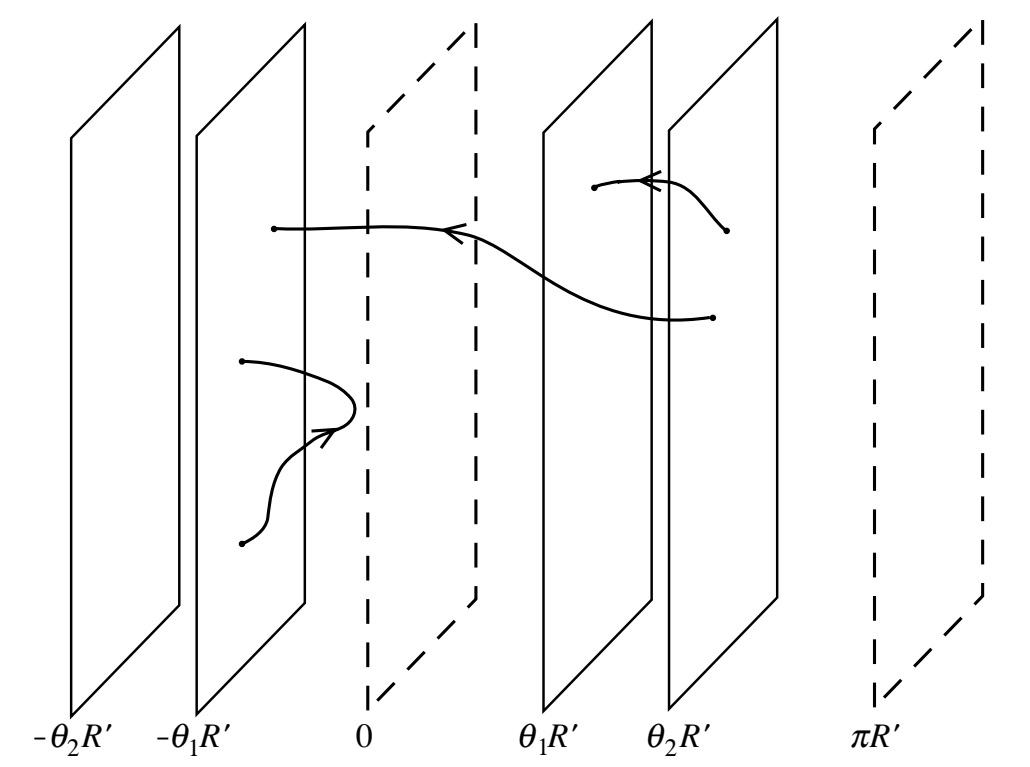
\includegraphics[width=0.6\textwidth,natwidth=721,natheight=555]{Fig8.7.jpg}
		\caption{定向形平面在0处和$\pi R^{\prime}$处, D-膜在$\theta_{1} R^{\prime}$ 和 $\theta_{2} R^{\prime}$处, 
		而D-膜镜像在$-\theta_{1} R^{\prime}$ 和 $-\theta_{2} R^{\prime}$处. 扭挠算符 $\Omega$ 在任何弦上的作用是时空反转的一个组合以及反转定向箭头. 
		%so that the string running from 2 to the image of 1 becomes a string running from 1 to the image of 2.
		}\label{Fig8.7}
	\end{center}
\end{figure}


如果$n$是奇数, $W$ 的最后一个本征值是$\pm 1$, 使得在 $T$-对偶图景中, 固定在两个定向面中的一个. 没有镜像, 这实际是半D-膜. 
另外如果我们考察 $n=2$ 的威尔逊线 $\operatorname{diag}(1,-1)$ (这在 $O(2)$ 而非 $SO(2)$ 中), 那么出现的就不是一个D-膜和它的像, 而是两个半D膜.

同D-膜一样, 定向平面会与伸缩子和度规耦合. 振幅与上节相同, 只不过要用 Klein 瓶和 Möbius 带替换圆环. 
实际上, 我们已经在第\ref{cha:7}章做过相关计算. 在那里我们发现总伸缩子耦合对于$S O\left(2^{13}\right)$抵消了. 
在$T$-对偶图景中, $2^{12}$ 个D-膜的总伸缩子耦合抵消了 (镜像未参与计数). 如果我们对$k=25-p$个维度紧致化, 就会有 $2^{k}$个不动平面, 
它们的坐标是0和$\pi R_{m}^{\prime}$的所有组合. 因此单个不动平面的有效作用量是
\begin{equation}
	2^{12-k} T_{p} \int \dif^{p+1} \xi \: \me^{-\Phi} (-\operatorname{det} G_{ab})^{1/2} \:, \label{8.8.5}
\end{equation}
积分跑遍不动平面.

尽管定向形没有扭挠分区的直接类比, 但是某种意义下, 扭态是开弦. 既然这个类比不是完全的, 我们不倾向于强调这一点: 
规范化 $\Omega$ 自身并不引入世界面边界. 然而, 在定向形理论中加入开弦, 以抵消伸缩子蝌蚪, 却有一定的物理意义. 这个抵消在超弦中将扮演重要角色.
